\documentclass[twoside]{book}

% Packages required by doxygen
\usepackage{fixltx2e}
\usepackage{calc}
\usepackage{doxygen}
\usepackage[export]{adjustbox} % also loads graphicx
\usepackage{graphicx}
\usepackage[utf8]{inputenc}
\usepackage{makeidx}
\usepackage{multicol}
\usepackage{multirow}
\PassOptionsToPackage{warn}{textcomp}
\usepackage{textcomp}
\usepackage[nointegrals]{wasysym}
\usepackage[table]{xcolor}

% NLS support packages
\usepackage[french]{babel}

% Font selection
\usepackage[T1]{fontenc}
\usepackage[scaled=.90]{helvet}
\usepackage{courier}
\usepackage{amssymb}
\usepackage{sectsty}
\renewcommand{\familydefault}{\sfdefault}
\allsectionsfont{%
  \fontseries{bc}\selectfont%
  \color{darkgray}%
}
\renewcommand{\DoxyLabelFont}{%
  \fontseries{bc}\selectfont%
  \color{darkgray}%
}
\newcommand{\+}{\discretionary{\mbox{\scriptsize$\hookleftarrow$}}{}{}}

% Page & text layout
\usepackage{geometry}
\geometry{%
  a4paper,%
  top=2.5cm,%
  bottom=2.5cm,%
  left=2.5cm,%
  right=2.5cm%
}
\tolerance=750
\hfuzz=15pt
\hbadness=750
\setlength{\emergencystretch}{15pt}
\setlength{\parindent}{0cm}
\setlength{\parskip}{3ex plus 2ex minus 2ex}
\makeatletter
\renewcommand{\paragraph}{%
  \@startsection{paragraph}{4}{0ex}{-1.0ex}{1.0ex}{%
    \normalfont\normalsize\bfseries\SS@parafont%
  }%
}
\renewcommand{\subparagraph}{%
  \@startsection{subparagraph}{5}{0ex}{-1.0ex}{1.0ex}{%
    \normalfont\normalsize\bfseries\SS@subparafont%
  }%
}
\makeatother

% Headers & footers
\usepackage{fancyhdr}
\pagestyle{fancyplain}
\fancyhead[LE]{\fancyplain{}{\bfseries\thepage}}
\fancyhead[CE]{\fancyplain{}{}}
\fancyhead[RE]{\fancyplain{}{\bfseries\leftmark}}
\fancyhead[LO]{\fancyplain{}{\bfseries\rightmark}}
\fancyhead[CO]{\fancyplain{}{}}
\fancyhead[RO]{\fancyplain{}{\bfseries\thepage}}
\fancyfoot[LE]{\fancyplain{}{}}
\fancyfoot[CE]{\fancyplain{}{}}
\fancyfoot[RE]{\fancyplain{}{\bfseries\scriptsize Généré par Doxygen }}
\fancyfoot[LO]{\fancyplain{}{\bfseries\scriptsize Généré par Doxygen }}
\fancyfoot[CO]{\fancyplain{}{}}
\fancyfoot[RO]{\fancyplain{}{}}
\renewcommand{\footrulewidth}{0.4pt}
\renewcommand{\chaptermark}[1]{%
  \markboth{#1}{}%
}
\renewcommand{\sectionmark}[1]{%
  \markright{\thesection\ #1}%
}

% Indices & bibliography
\usepackage{natbib}
\usepackage[titles]{tocloft}
\setcounter{tocdepth}{3}
\setcounter{secnumdepth}{5}
\makeindex

% Hyperlinks (required, but should be loaded last)
\usepackage{ifpdf}
\ifpdf
  \usepackage[pdftex,pagebackref=true]{hyperref}
\else
  \usepackage[ps2pdf,pagebackref=true]{hyperref}
\fi
\hypersetup{%
  colorlinks=true,%
  linkcolor=blue,%
  citecolor=blue,%
  unicode%
}

% Custom commands
\newcommand{\clearemptydoublepage}{%
  \newpage{\pagestyle{empty}\cleardoublepage}%
}

\usepackage{caption}
\captionsetup{labelsep=space,justification=centering,font={bf},singlelinecheck=off,skip=4pt,position=top}

%===== C O N T E N T S =====

\begin{document}

% Titlepage & ToC
\hypersetup{pageanchor=false,
             bookmarksnumbered=true,
             pdfencoding=unicode
            }
\pagenumbering{alph}
\begin{titlepage}
\vspace*{7cm}
\begin{center}%
{\Large A\+I\+B\+Attle\+Simulator3000 }\\
\vspace*{1cm}
{\large Généré par Doxygen 1.8.13}\\
\end{center}
\end{titlepage}
\clearemptydoublepage
\pagenumbering{roman}
\tableofcontents
\clearemptydoublepage
\pagenumbering{arabic}
\hypersetup{pageanchor=true}

%--- Begin generated contents ---
\chapter{Index des espaces de nommage}
\section{Liste des espaces de nommage}
Liste de tous les espaces de nommage avec une brève description\+:\begin{DoxyCompactList}
\item\contentsline{section}{\hyperlink{namespaceAttackType}{Attack\+Type} }{\pageref{namespaceAttackType}}{}
\item\contentsline{section}{\hyperlink{namespaceDirection}{Direction} }{\pageref{namespaceDirection}}{}
\item\contentsline{section}{\hyperlink{namespaceDommageType}{Dommage\+Type} }{\pageref{namespaceDommageType}}{}
\end{DoxyCompactList}

\chapter{Index hiérarchique}
\section{Hiérarchie des classes}
Cette liste d\textquotesingle{}héritage est classée approximativement par ordre alphabétique \+:\begin{DoxyCompactList}
\item \contentsline{section}{Component}{\pageref{structComponent}}{}
\begin{DoxyCompactList}
\item \contentsline{section}{Armor\+Component}{\pageref{structArmorComponent}}{}
\item \contentsline{section}{Attack\+Component}{\pageref{structAttackComponent}}{}
\item \contentsline{section}{Health\+Component}{\pageref{structHealthComponent}}{}
\item \contentsline{section}{Position\+Component}{\pageref{structPositionComponent}}{}
\item \contentsline{section}{Speed\+Component}{\pageref{structSpeedComponent}}{}
\end{DoxyCompactList}
\item \contentsline{section}{Component\+Storer}{\pageref{classComponentStorer}}{}
\item \contentsline{section}{Entity\+Manager}{\pageref{classEntityManager}}{}
\item \contentsline{section}{Lua\+Script}{\pageref{classLuaScript}}{}
\item \contentsline{section}{Position}{\pageref{structPosition}}{}
\item \contentsline{section}{Visitor}{\pageref{classVisitor}}{}
\begin{DoxyCompactList}
\item \contentsline{section}{Entity\+Creator}{\pageref{classEntityCreator}}{}
\item \contentsline{section}{Move\+System}{\pageref{classMoveSystem}}{}
\end{DoxyCompactList}
\end{DoxyCompactList}

\chapter{Index des classes}
\section{Liste des classes}
Liste des classes, structures, unions et interfaces avec une brève description \+:\begin{DoxyCompactList}
\item\contentsline{section}{\hyperlink{structArmorComponent}{Armor\+Component} }{\pageref{structArmorComponent}}{}
\item\contentsline{section}{\hyperlink{structAttackComponent}{Attack\+Component} }{\pageref{structAttackComponent}}{}
\item\contentsline{section}{\hyperlink{structComponent}{Component} \\*Classe de base pour les composant }{\pageref{structComponent}}{}
\item\contentsline{section}{\hyperlink{classComponentStorer}{Component\+Storer} }{\pageref{classComponentStorer}}{}
\item\contentsline{section}{\hyperlink{classEntityCreator}{Entity\+Creator} \\*Cette classe a pour but de creer les entites sur demande }{\pageref{classEntityCreator}}{}
\item\contentsline{section}{\hyperlink{classEntityManager}{Entity\+Manager} }{\pageref{classEntityManager}}{}
\item\contentsline{section}{\hyperlink{structHealthComponent}{Health\+Component} }{\pageref{structHealthComponent}}{}
\item\contentsline{section}{\hyperlink{classLuaScript}{Lua\+Script} }{\pageref{classLuaScript}}{}
\item\contentsline{section}{\hyperlink{classMoveSystem}{Move\+System} }{\pageref{classMoveSystem}}{}
\item\contentsline{section}{\hyperlink{structPosition}{Position} }{\pageref{structPosition}}{}
\item\contentsline{section}{\hyperlink{structPositionComponent}{Position\+Component} }{\pageref{structPositionComponent}}{}
\item\contentsline{section}{\hyperlink{structSpeedComponent}{Speed\+Component} }{\pageref{structSpeedComponent}}{}
\item\contentsline{section}{\hyperlink{classVisitor}{Visitor} }{\pageref{classVisitor}}{}
\end{DoxyCompactList}

\chapter{Index des fichiers}
\section{Liste des fichiers}
Liste de tous les fichiers avec une brève description \+:\begin{DoxyCompactList}
\item\contentsline{section}{include/\hyperlink{Component_8hpp}{Component.\+hpp} \\*Ici sont declares les class \hyperlink{classVisitor}{Visitor}, \hyperlink{structComponent}{Component} et les class filles de component }{\pageref{Component_8hpp}}{}
\item\contentsline{section}{include/\hyperlink{ComponentStorer_8hpp}{Component\+Storer.\+hpp} }{\pageref{ComponentStorer_8hpp}}{}
\item\contentsline{section}{include/\hyperlink{Define_8hpp}{Define.\+hpp} }{\pageref{Define_8hpp}}{}
\item\contentsline{section}{include/\hyperlink{ECS_8hpp}{E\+C\+S.\+hpp} }{\pageref{ECS_8hpp}}{}
\item\contentsline{section}{include/\hyperlink{ECSEntity_8hpp}{E\+C\+S\+Entity.\+hpp} }{\pageref{ECSEntity_8hpp}}{}
\item\contentsline{section}{include/\hyperlink{EntityCreator_8hpp}{Entity\+Creator.\+hpp} \\*Ici est declare la class \hyperlink{classEntityCreator}{Entity\+Creator} }{\pageref{EntityCreator_8hpp}}{}
\item\contentsline{section}{include/\hyperlink{EntityManager_8hpp}{Entity\+Manager.\+hpp} }{\pageref{EntityManager_8hpp}}{}
\item\contentsline{section}{include/\hyperlink{LuaScript_8hpp}{Lua\+Script.\+hpp} }{\pageref{LuaScript_8hpp}}{}
\item\contentsline{section}{include/\hyperlink{MoveSystem_8hpp}{Move\+System.\+hpp} }{\pageref{MoveSystem_8hpp}}{}
\item\contentsline{section}{src/\hyperlink{Component_8cpp}{Component.\+cpp} }{\pageref{Component_8cpp}}{}
\item\contentsline{section}{src/\hyperlink{ComponentStorer_8cpp}{Component\+Storer.\+cpp} }{\pageref{ComponentStorer_8cpp}}{}
\item\contentsline{section}{src/\hyperlink{Define_8cpp}{Define.\+cpp} }{\pageref{Define_8cpp}}{}
\item\contentsline{section}{src/\hyperlink{EntityCreator_8cpp}{Entity\+Creator.\+cpp} }{\pageref{EntityCreator_8cpp}}{}
\item\contentsline{section}{src/\hyperlink{EntityManager_8cpp}{Entity\+Manager.\+cpp} }{\pageref{EntityManager_8cpp}}{}
\item\contentsline{section}{src/\hyperlink{LuaScript_8cpp}{Lua\+Script.\+cpp} }{\pageref{LuaScript_8cpp}}{}
\item\contentsline{section}{src/\hyperlink{main_8cpp}{main.\+cpp} }{\pageref{main_8cpp}}{}
\item\contentsline{section}{src/\hyperlink{MoveSystem_8cpp}{Move\+System.\+cpp} }{\pageref{MoveSystem_8cpp}}{}
\end{DoxyCompactList}

\chapter{Documentation des espaces de nommage}
\hypertarget{namespaceAttackType}{}\section{Référence de l\textquotesingle{}espace de nommage Attack\+Type}
\label{namespaceAttackType}\index{Attack\+Type@{Attack\+Type}}
\subsection*{Énumérations}
\begin{DoxyCompactItemize}
\item 
enum \hyperlink{namespaceAttackType_a26a2d73c5f73a06a63a568dcd519d302}{Type} \{ \hyperlink{namespaceAttackType_a26a2d73c5f73a06a63a568dcd519d302a53add169c04afbf920774a3cdf710106}{Melee}, 
\hyperlink{namespaceAttackType_a26a2d73c5f73a06a63a568dcd519d302a3a9ed6c6d45ca13d8df01c12f7d538fd}{Distance}, 
\hyperlink{namespaceAttackType_a26a2d73c5f73a06a63a568dcd519d302a73b8be32d0bc40ff4a231436e331f161}{N\+O\+NE}
 \}
\end{DoxyCompactItemize}
\subsection*{Variables}
\begin{DoxyCompactItemize}
\item 
const std\+::array$<$ \hyperlink{namespaceAttackType_a26a2d73c5f73a06a63a568dcd519d302}{Type}, 2 $>$ \hyperlink{namespaceAttackType_a44c88a70d0a57861180381c34bda18e9}{All} = \{\hyperlink{namespaceAttackType_a26a2d73c5f73a06a63a568dcd519d302a53add169c04afbf920774a3cdf710106}{Melee}, \hyperlink{namespaceAttackType_a26a2d73c5f73a06a63a568dcd519d302a3a9ed6c6d45ca13d8df01c12f7d538fd}{Distance}\}
\end{DoxyCompactItemize}


\subsection{Documentation du type de l\textquotesingle{}énumération}
\mbox{\Hypertarget{namespaceAttackType_a26a2d73c5f73a06a63a568dcd519d302}\label{namespaceAttackType_a26a2d73c5f73a06a63a568dcd519d302}} 
\index{Attack\+Type@{Attack\+Type}!Type@{Type}}
\index{Type@{Type}!Attack\+Type@{Attack\+Type}}
\subsubsection{\texorpdfstring{Type}{Type}}
{\footnotesize\ttfamily enum \hyperlink{namespaceAttackType_a26a2d73c5f73a06a63a568dcd519d302}{Attack\+Type\+::\+Type}}

\begin{DoxyEnumFields}{Valeurs énumérées}
\raisebox{\heightof{T}}[0pt][0pt]{\index{Melee@{Melee}!Attack\+Type@{Attack\+Type}}\index{Attack\+Type@{Attack\+Type}!Melee@{Melee}}}\mbox{\Hypertarget{namespaceAttackType_a26a2d73c5f73a06a63a568dcd519d302a53add169c04afbf920774a3cdf710106}\label{namespaceAttackType_a26a2d73c5f73a06a63a568dcd519d302a53add169c04afbf920774a3cdf710106}} 
Melee&\\
\hline

\raisebox{\heightof{T}}[0pt][0pt]{\index{Distance@{Distance}!Attack\+Type@{Attack\+Type}}\index{Attack\+Type@{Attack\+Type}!Distance@{Distance}}}\mbox{\Hypertarget{namespaceAttackType_a26a2d73c5f73a06a63a568dcd519d302a3a9ed6c6d45ca13d8df01c12f7d538fd}\label{namespaceAttackType_a26a2d73c5f73a06a63a568dcd519d302a3a9ed6c6d45ca13d8df01c12f7d538fd}} 
Distance&\\
\hline

\raisebox{\heightof{T}}[0pt][0pt]{\index{N\+O\+NE@{N\+O\+NE}!Attack\+Type@{Attack\+Type}}\index{Attack\+Type@{Attack\+Type}!N\+O\+NE@{N\+O\+NE}}}\mbox{\Hypertarget{namespaceAttackType_a26a2d73c5f73a06a63a568dcd519d302a73b8be32d0bc40ff4a231436e331f161}\label{namespaceAttackType_a26a2d73c5f73a06a63a568dcd519d302a73b8be32d0bc40ff4a231436e331f161}} 
N\+O\+NE&\\
\hline

\end{DoxyEnumFields}


\subsection{Documentation des variables}
\mbox{\Hypertarget{namespaceAttackType_a44c88a70d0a57861180381c34bda18e9}\label{namespaceAttackType_a44c88a70d0a57861180381c34bda18e9}} 
\index{Attack\+Type@{Attack\+Type}!All@{All}}
\index{All@{All}!Attack\+Type@{Attack\+Type}}
\subsubsection{\texorpdfstring{All}{All}}
{\footnotesize\ttfamily const std\+::array$<$\hyperlink{namespaceAttackType_a26a2d73c5f73a06a63a568dcd519d302}{Type}, 2$>$ Attack\+Type\+::\+All = \{\hyperlink{namespaceAttackType_a26a2d73c5f73a06a63a568dcd519d302a53add169c04afbf920774a3cdf710106}{Melee}, \hyperlink{namespaceAttackType_a26a2d73c5f73a06a63a568dcd519d302a3a9ed6c6d45ca13d8df01c12f7d538fd}{Distance}\}}


\hypertarget{namespaceDirection}{}\section{Référence de l\textquotesingle{}espace de nommage Direction}
\label{namespaceDirection}\index{Direction@{Direction}}
\subsection*{Énumérations}
\begin{DoxyCompactItemize}
\item 
enum \hyperlink{namespaceDirection_aaa56ca1cc2883e1cab31b6cbb5054418}{Dir} \{ \newline
\hyperlink{namespaceDirection_aaa56ca1cc2883e1cab31b6cbb5054418a2dcf8e71283b05e59e3b7d1fa4228623}{Up}, 
\hyperlink{namespaceDirection_aaa56ca1cc2883e1cab31b6cbb5054418aad5dbfe9b746123d7af7381b52a183f1}{Down}, 
\hyperlink{namespaceDirection_aaa56ca1cc2883e1cab31b6cbb5054418aa6314d583c5d1432de99eb3fda30bdea}{Left}, 
\hyperlink{namespaceDirection_aaa56ca1cc2883e1cab31b6cbb5054418a1d010c1da83b45aa3ded2cb937d2d979}{Right}, 
\newline
\hyperlink{namespaceDirection_aaa56ca1cc2883e1cab31b6cbb5054418a1f9c924b3a1502e5e35ed148994c4148}{None}
 \}
\end{DoxyCompactItemize}
\subsection*{Variables}
\begin{DoxyCompactItemize}
\item 
const std\+::array$<$ \hyperlink{namespaceDirection_aaa56ca1cc2883e1cab31b6cbb5054418}{Dir}, 4 $>$ \hyperlink{namespaceDirection_aabd5fd5d609f7dda7f8f50f1dbd563a7}{All} = \{\hyperlink{namespaceDirection_aaa56ca1cc2883e1cab31b6cbb5054418a2dcf8e71283b05e59e3b7d1fa4228623}{Up}, \hyperlink{namespaceDirection_aaa56ca1cc2883e1cab31b6cbb5054418aad5dbfe9b746123d7af7381b52a183f1}{Down}, \hyperlink{namespaceDirection_aaa56ca1cc2883e1cab31b6cbb5054418aa6314d583c5d1432de99eb3fda30bdea}{Left}, \hyperlink{namespaceDirection_aaa56ca1cc2883e1cab31b6cbb5054418a1d010c1da83b45aa3ded2cb937d2d979}{Right}\}
\end{DoxyCompactItemize}


\subsection{Documentation du type de l\textquotesingle{}énumération}
\mbox{\Hypertarget{namespaceDirection_aaa56ca1cc2883e1cab31b6cbb5054418}\label{namespaceDirection_aaa56ca1cc2883e1cab31b6cbb5054418}} 
\index{Direction@{Direction}!Dir@{Dir}}
\index{Dir@{Dir}!Direction@{Direction}}
\subsubsection{\texorpdfstring{Dir}{Dir}}
{\footnotesize\ttfamily enum \hyperlink{namespaceDirection_aaa56ca1cc2883e1cab31b6cbb5054418}{Direction\+::\+Dir}}

\begin{DoxyEnumFields}{Valeurs énumérées}
\raisebox{\heightof{T}}[0pt][0pt]{\index{Up@{Up}!Direction@{Direction}}\index{Direction@{Direction}!Up@{Up}}}\mbox{\Hypertarget{namespaceDirection_aaa56ca1cc2883e1cab31b6cbb5054418a2dcf8e71283b05e59e3b7d1fa4228623}\label{namespaceDirection_aaa56ca1cc2883e1cab31b6cbb5054418a2dcf8e71283b05e59e3b7d1fa4228623}} 
Up&\\
\hline

\raisebox{\heightof{T}}[0pt][0pt]{\index{Down@{Down}!Direction@{Direction}}\index{Direction@{Direction}!Down@{Down}}}\mbox{\Hypertarget{namespaceDirection_aaa56ca1cc2883e1cab31b6cbb5054418aad5dbfe9b746123d7af7381b52a183f1}\label{namespaceDirection_aaa56ca1cc2883e1cab31b6cbb5054418aad5dbfe9b746123d7af7381b52a183f1}} 
Down&\\
\hline

\raisebox{\heightof{T}}[0pt][0pt]{\index{Left@{Left}!Direction@{Direction}}\index{Direction@{Direction}!Left@{Left}}}\mbox{\Hypertarget{namespaceDirection_aaa56ca1cc2883e1cab31b6cbb5054418aa6314d583c5d1432de99eb3fda30bdea}\label{namespaceDirection_aaa56ca1cc2883e1cab31b6cbb5054418aa6314d583c5d1432de99eb3fda30bdea}} 
Left&\\
\hline

\raisebox{\heightof{T}}[0pt][0pt]{\index{Right@{Right}!Direction@{Direction}}\index{Direction@{Direction}!Right@{Right}}}\mbox{\Hypertarget{namespaceDirection_aaa56ca1cc2883e1cab31b6cbb5054418a1d010c1da83b45aa3ded2cb937d2d979}\label{namespaceDirection_aaa56ca1cc2883e1cab31b6cbb5054418a1d010c1da83b45aa3ded2cb937d2d979}} 
Right&\\
\hline

\raisebox{\heightof{T}}[0pt][0pt]{\index{None@{None}!Direction@{Direction}}\index{Direction@{Direction}!None@{None}}}\mbox{\Hypertarget{namespaceDirection_aaa56ca1cc2883e1cab31b6cbb5054418a1f9c924b3a1502e5e35ed148994c4148}\label{namespaceDirection_aaa56ca1cc2883e1cab31b6cbb5054418a1f9c924b3a1502e5e35ed148994c4148}} 
None&\\
\hline

\end{DoxyEnumFields}


\subsection{Documentation des variables}
\mbox{\Hypertarget{namespaceDirection_aabd5fd5d609f7dda7f8f50f1dbd563a7}\label{namespaceDirection_aabd5fd5d609f7dda7f8f50f1dbd563a7}} 
\index{Direction@{Direction}!All@{All}}
\index{All@{All}!Direction@{Direction}}
\subsubsection{\texorpdfstring{All}{All}}
{\footnotesize\ttfamily const std\+::array$<$\hyperlink{namespaceDirection_aaa56ca1cc2883e1cab31b6cbb5054418}{Dir}, 4$>$ Direction\+::\+All = \{\hyperlink{namespaceDirection_aaa56ca1cc2883e1cab31b6cbb5054418a2dcf8e71283b05e59e3b7d1fa4228623}{Up}, \hyperlink{namespaceDirection_aaa56ca1cc2883e1cab31b6cbb5054418aad5dbfe9b746123d7af7381b52a183f1}{Down}, \hyperlink{namespaceDirection_aaa56ca1cc2883e1cab31b6cbb5054418aa6314d583c5d1432de99eb3fda30bdea}{Left}, \hyperlink{namespaceDirection_aaa56ca1cc2883e1cab31b6cbb5054418a1d010c1da83b45aa3ded2cb937d2d979}{Right}\}}


\hypertarget{namespaceDommageType}{}\section{Référence de l\textquotesingle{}espace de nommage Dommage\+Type}
\label{namespaceDommageType}\index{Dommage\+Type@{Dommage\+Type}}
\subsection*{Énumérations}
\begin{DoxyCompactItemize}
\item 
enum \hyperlink{namespaceDommageType_a6e5dff665b7631fe6ec9065dddbebcfd}{Type} \{ \hyperlink{namespaceDommageType_a6e5dff665b7631fe6ec9065dddbebcfdabca33f1e8d86b9faddd26010eb172ec0}{Pierce}, 
\hyperlink{namespaceDommageType_a6e5dff665b7631fe6ec9065dddbebcfdad7195516d2e659e73c0f22e64249517b}{Shock}, 
\hyperlink{namespaceDommageType_a6e5dff665b7631fe6ec9065dddbebcfdab12cf1b0c6c2cd00d9466c6cab208137}{Magic}, 
\hyperlink{namespaceDommageType_a6e5dff665b7631fe6ec9065dddbebcfda11352066c669cc04a816c1fbc404eb5f}{N\+O\+NE}
 \}
\end{DoxyCompactItemize}
\subsection*{Variables}
\begin{DoxyCompactItemize}
\item 
const std\+::array$<$ \hyperlink{namespaceDommageType_a6e5dff665b7631fe6ec9065dddbebcfd}{Type}, 3 $>$ \hyperlink{namespaceDommageType_a95378d0bf91b2850a1a5c112c35bb75c}{All} = \{\hyperlink{namespaceDommageType_a6e5dff665b7631fe6ec9065dddbebcfdad7195516d2e659e73c0f22e64249517b}{Shock}, \hyperlink{namespaceDommageType_a6e5dff665b7631fe6ec9065dddbebcfdabca33f1e8d86b9faddd26010eb172ec0}{Pierce}, \hyperlink{namespaceDommageType_a6e5dff665b7631fe6ec9065dddbebcfdab12cf1b0c6c2cd00d9466c6cab208137}{Magic}\}
\end{DoxyCompactItemize}


\subsection{Documentation du type de l\textquotesingle{}énumération}
\mbox{\Hypertarget{namespaceDommageType_a6e5dff665b7631fe6ec9065dddbebcfd}\label{namespaceDommageType_a6e5dff665b7631fe6ec9065dddbebcfd}} 
\index{Dommage\+Type@{Dommage\+Type}!Type@{Type}}
\index{Type@{Type}!Dommage\+Type@{Dommage\+Type}}
\subsubsection{\texorpdfstring{Type}{Type}}
{\footnotesize\ttfamily enum \hyperlink{namespaceDommageType_a6e5dff665b7631fe6ec9065dddbebcfd}{Dommage\+Type\+::\+Type}}

\begin{DoxyEnumFields}{Valeurs énumérées}
\raisebox{\heightof{T}}[0pt][0pt]{\index{Pierce@{Pierce}!Dommage\+Type@{Dommage\+Type}}\index{Dommage\+Type@{Dommage\+Type}!Pierce@{Pierce}}}\mbox{\Hypertarget{namespaceDommageType_a6e5dff665b7631fe6ec9065dddbebcfdabca33f1e8d86b9faddd26010eb172ec0}\label{namespaceDommageType_a6e5dff665b7631fe6ec9065dddbebcfdabca33f1e8d86b9faddd26010eb172ec0}} 
Pierce&\\
\hline

\raisebox{\heightof{T}}[0pt][0pt]{\index{Shock@{Shock}!Dommage\+Type@{Dommage\+Type}}\index{Dommage\+Type@{Dommage\+Type}!Shock@{Shock}}}\mbox{\Hypertarget{namespaceDommageType_a6e5dff665b7631fe6ec9065dddbebcfdad7195516d2e659e73c0f22e64249517b}\label{namespaceDommageType_a6e5dff665b7631fe6ec9065dddbebcfdad7195516d2e659e73c0f22e64249517b}} 
Shock&\\
\hline

\raisebox{\heightof{T}}[0pt][0pt]{\index{Magic@{Magic}!Dommage\+Type@{Dommage\+Type}}\index{Dommage\+Type@{Dommage\+Type}!Magic@{Magic}}}\mbox{\Hypertarget{namespaceDommageType_a6e5dff665b7631fe6ec9065dddbebcfdab12cf1b0c6c2cd00d9466c6cab208137}\label{namespaceDommageType_a6e5dff665b7631fe6ec9065dddbebcfdab12cf1b0c6c2cd00d9466c6cab208137}} 
Magic&\\
\hline

\raisebox{\heightof{T}}[0pt][0pt]{\index{N\+O\+NE@{N\+O\+NE}!Dommage\+Type@{Dommage\+Type}}\index{Dommage\+Type@{Dommage\+Type}!N\+O\+NE@{N\+O\+NE}}}\mbox{\Hypertarget{namespaceDommageType_a6e5dff665b7631fe6ec9065dddbebcfda11352066c669cc04a816c1fbc404eb5f}\label{namespaceDommageType_a6e5dff665b7631fe6ec9065dddbebcfda11352066c669cc04a816c1fbc404eb5f}} 
N\+O\+NE&\\
\hline

\end{DoxyEnumFields}


\subsection{Documentation des variables}
\mbox{\Hypertarget{namespaceDommageType_a95378d0bf91b2850a1a5c112c35bb75c}\label{namespaceDommageType_a95378d0bf91b2850a1a5c112c35bb75c}} 
\index{Dommage\+Type@{Dommage\+Type}!All@{All}}
\index{All@{All}!Dommage\+Type@{Dommage\+Type}}
\subsubsection{\texorpdfstring{All}{All}}
{\footnotesize\ttfamily const std\+::array$<$\hyperlink{namespaceDommageType_a6e5dff665b7631fe6ec9065dddbebcfd}{Type}, 3$>$ Dommage\+Type\+::\+All = \{\hyperlink{namespaceDommageType_a6e5dff665b7631fe6ec9065dddbebcfdad7195516d2e659e73c0f22e64249517b}{Shock}, \hyperlink{namespaceDommageType_a6e5dff665b7631fe6ec9065dddbebcfdabca33f1e8d86b9faddd26010eb172ec0}{Pierce}, \hyperlink{namespaceDommageType_a6e5dff665b7631fe6ec9065dddbebcfdab12cf1b0c6c2cd00d9466c6cab208137}{Magic}\}}


\chapter{Documentation des classes}
\hypertarget{structArmorComponent}{}\section{Référence de la structure Armor\+Component}
\label{structArmorComponent}\index{Armor\+Component@{Armor\+Component}}


{\ttfamily \#include $<$Component.\+hpp$>$}

Graphe d\textquotesingle{}héritage de Armor\+Component\+:\begin{figure}[H]
\begin{center}
\leavevmode
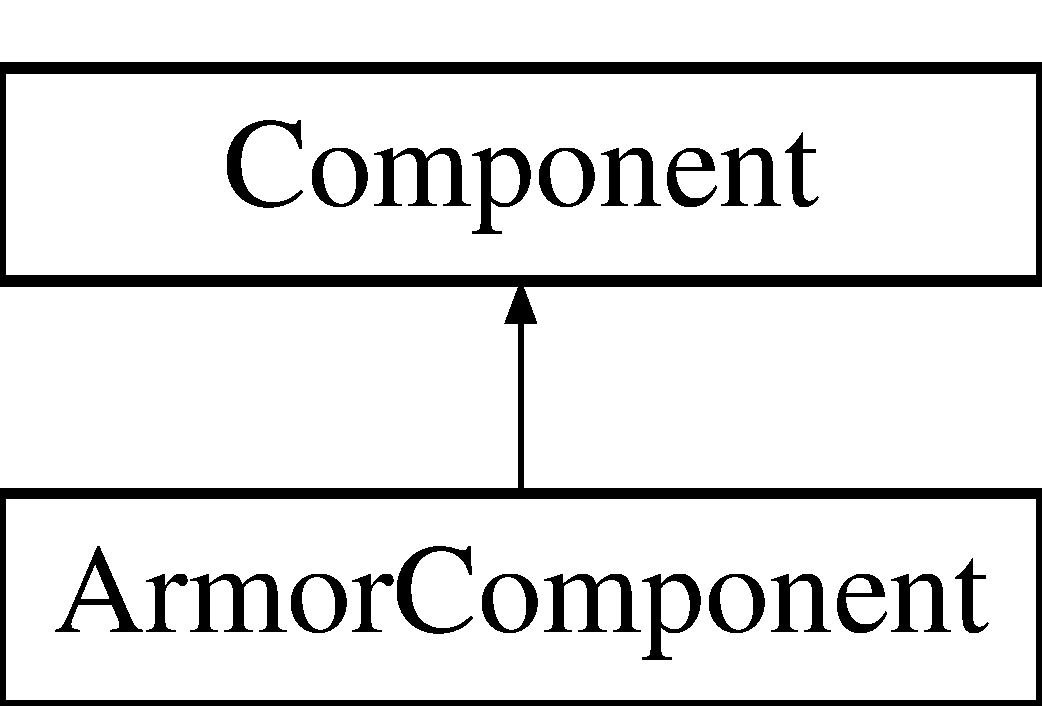
\includegraphics[height=2.000000cm]{structArmorComponent}
\end{center}
\end{figure}
\subsection*{Fonctions membres publiques}
\begin{DoxyCompactItemize}
\item 
\hyperlink{structArmorComponent_a836b3a9a30b3445c3abf3a7b4e56707c}{Armor\+Component} (int p, int s, int m)
\item 
virtual void \hyperlink{structArmorComponent_aac5863d4195fe056fbb0a2a0af17b6e0}{accept} (\hyperlink{classVisitor}{Visitor} \&v)
\end{DoxyCompactItemize}
\subsection*{Attributs publics}
\begin{DoxyCompactItemize}
\item 
int \hyperlink{structArmorComponent_ac039e03a0e2377aff82d95c317777ec7}{pierce\+Armor}
\item 
int \hyperlink{structArmorComponent_a2ece22c73ce63988ea38644fb1d856c5}{shock\+Armor}
\item 
int \hyperlink{structArmorComponent_a88e4b9e35be500896af52d24942e7465}{magic\+Armor}
\end{DoxyCompactItemize}


\subsection{Documentation des constructeurs et destructeur}
\mbox{\Hypertarget{structArmorComponent_a836b3a9a30b3445c3abf3a7b4e56707c}\label{structArmorComponent_a836b3a9a30b3445c3abf3a7b4e56707c}} 
\index{Armor\+Component@{Armor\+Component}!Armor\+Component@{Armor\+Component}}
\index{Armor\+Component@{Armor\+Component}!Armor\+Component@{Armor\+Component}}
\subsubsection{\texorpdfstring{Armor\+Component()}{ArmorComponent()}}
{\footnotesize\ttfamily Armor\+Component\+::\+Armor\+Component (\begin{DoxyParamCaption}\item[{int}]{p,  }\item[{int}]{s,  }\item[{int}]{m }\end{DoxyParamCaption})\hspace{0.3cm}{\ttfamily [inline]}}



\subsection{Documentation des fonctions membres}
\mbox{\Hypertarget{structArmorComponent_aac5863d4195fe056fbb0a2a0af17b6e0}\label{structArmorComponent_aac5863d4195fe056fbb0a2a0af17b6e0}} 
\index{Armor\+Component@{Armor\+Component}!accept@{accept}}
\index{accept@{accept}!Armor\+Component@{Armor\+Component}}
\subsubsection{\texorpdfstring{accept()}{accept()}}
{\footnotesize\ttfamily void Armor\+Component\+::accept (\begin{DoxyParamCaption}\item[{\hyperlink{classVisitor}{Visitor} \&}]{v }\end{DoxyParamCaption})\hspace{0.3cm}{\ttfamily [virtual]}}

Fonction acceptant un visiteur


\begin{DoxyParams}{Paramètres}
{\em V} & le visiteur qui va etre accepter \\
\hline
\end{DoxyParams}


Implémente \hyperlink{structComponent_a1d42068fda4a9bf6571810f669b3bb21}{Component}.



\subsection{Documentation des données membres}
\mbox{\Hypertarget{structArmorComponent_a88e4b9e35be500896af52d24942e7465}\label{structArmorComponent_a88e4b9e35be500896af52d24942e7465}} 
\index{Armor\+Component@{Armor\+Component}!magic\+Armor@{magic\+Armor}}
\index{magic\+Armor@{magic\+Armor}!Armor\+Component@{Armor\+Component}}
\subsubsection{\texorpdfstring{magic\+Armor}{magicArmor}}
{\footnotesize\ttfamily int Armor\+Component\+::magic\+Armor}

\mbox{\Hypertarget{structArmorComponent_ac039e03a0e2377aff82d95c317777ec7}\label{structArmorComponent_ac039e03a0e2377aff82d95c317777ec7}} 
\index{Armor\+Component@{Armor\+Component}!pierce\+Armor@{pierce\+Armor}}
\index{pierce\+Armor@{pierce\+Armor}!Armor\+Component@{Armor\+Component}}
\subsubsection{\texorpdfstring{pierce\+Armor}{pierceArmor}}
{\footnotesize\ttfamily int Armor\+Component\+::pierce\+Armor}

\mbox{\Hypertarget{structArmorComponent_a2ece22c73ce63988ea38644fb1d856c5}\label{structArmorComponent_a2ece22c73ce63988ea38644fb1d856c5}} 
\index{Armor\+Component@{Armor\+Component}!shock\+Armor@{shock\+Armor}}
\index{shock\+Armor@{shock\+Armor}!Armor\+Component@{Armor\+Component}}
\subsubsection{\texorpdfstring{shock\+Armor}{shockArmor}}
{\footnotesize\ttfamily int Armor\+Component\+::shock\+Armor}



La documentation de cette structure a été générée à partir des fichiers suivants \+:\begin{DoxyCompactItemize}
\item 
include/\hyperlink{Component_8hpp}{Component.\+hpp}\item 
src/\hyperlink{Component_8cpp}{Component.\+cpp}\end{DoxyCompactItemize}

\hypertarget{structAttackComponent}{}\section{Référence de la structure Attack\+Component}
\label{structAttackComponent}\index{Attack\+Component@{Attack\+Component}}


{\ttfamily \#include $<$Component.\+hpp$>$}

Graphe d\textquotesingle{}héritage de Attack\+Component\+:\begin{figure}[H]
\begin{center}
\leavevmode
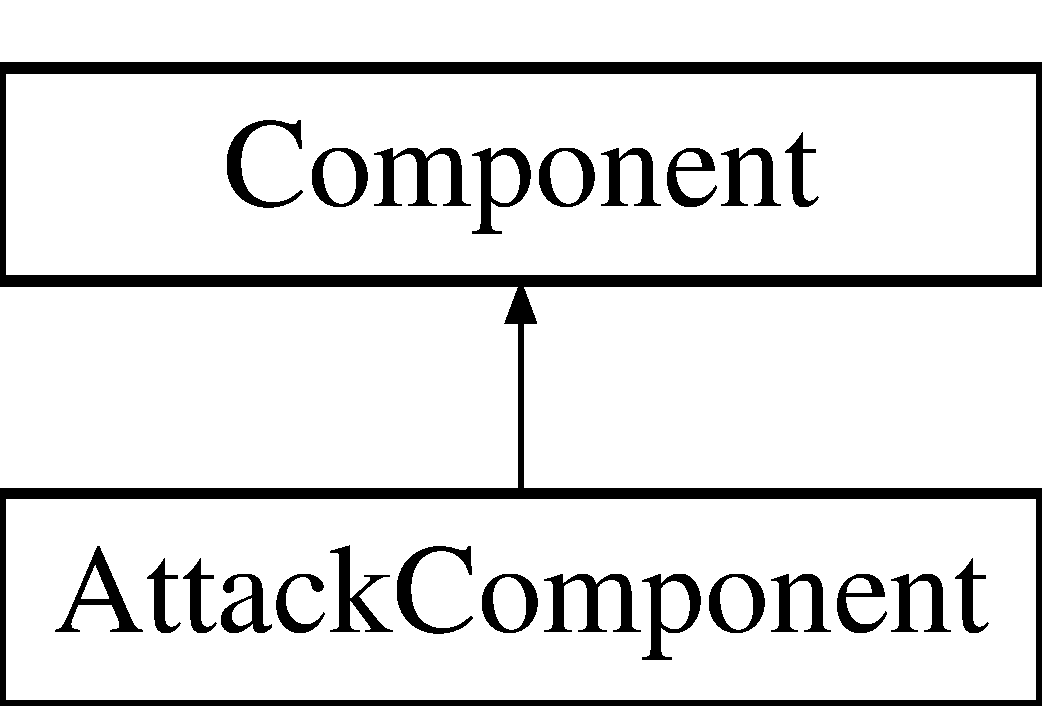
\includegraphics[height=2.000000cm]{structAttackComponent}
\end{center}
\end{figure}
\subsection*{Fonctions membres publiques}
\begin{DoxyCompactItemize}
\item 
\hyperlink{structAttackComponent_ab4d5e046930665a69f073554c3fad965}{Attack\+Component} (int a, \hyperlink{namespaceDommageType_a6e5dff665b7631fe6ec9065dddbebcfd}{Dommage\+Type\+::\+Type} d, \hyperlink{namespaceAttackType_a26a2d73c5f73a06a63a568dcd519d302}{Attack\+Type\+::\+Type} at)
\item 
virtual void \hyperlink{structAttackComponent_a6644fff9ad3be5bc7cd9571f811fe25e}{accept} (\hyperlink{classVisitor}{Visitor} \&v)
\end{DoxyCompactItemize}
\subsection*{Attributs publics}
\begin{DoxyCompactItemize}
\item 
int \hyperlink{structAttackComponent_a7af6243b23e8bdfec8eb75e267622b57}{amount}
\item 
\hyperlink{namespaceDommageType_a6e5dff665b7631fe6ec9065dddbebcfd}{Dommage\+Type\+::\+Type} \hyperlink{structAttackComponent_a324ca9d4107c8f2855d06a845228d29d}{dommage\+Type}
\item 
\hyperlink{namespaceAttackType_a26a2d73c5f73a06a63a568dcd519d302}{Attack\+Type\+::\+Type} \hyperlink{structAttackComponent_a672c95806b4aad77f6b0aaee6895611f}{attack\+Type}
\end{DoxyCompactItemize}


\subsection{Documentation des constructeurs et destructeur}
\mbox{\Hypertarget{structAttackComponent_ab4d5e046930665a69f073554c3fad965}\label{structAttackComponent_ab4d5e046930665a69f073554c3fad965}} 
\index{Attack\+Component@{Attack\+Component}!Attack\+Component@{Attack\+Component}}
\index{Attack\+Component@{Attack\+Component}!Attack\+Component@{Attack\+Component}}
\subsubsection{\texorpdfstring{Attack\+Component()}{AttackComponent()}}
{\footnotesize\ttfamily Attack\+Component\+::\+Attack\+Component (\begin{DoxyParamCaption}\item[{int}]{a,  }\item[{\hyperlink{namespaceDommageType_a6e5dff665b7631fe6ec9065dddbebcfd}{Dommage\+Type\+::\+Type}}]{d,  }\item[{\hyperlink{namespaceAttackType_a26a2d73c5f73a06a63a568dcd519d302}{Attack\+Type\+::\+Type}}]{at }\end{DoxyParamCaption})\hspace{0.3cm}{\ttfamily [inline]}}



\subsection{Documentation des fonctions membres}
\mbox{\Hypertarget{structAttackComponent_a6644fff9ad3be5bc7cd9571f811fe25e}\label{structAttackComponent_a6644fff9ad3be5bc7cd9571f811fe25e}} 
\index{Attack\+Component@{Attack\+Component}!accept@{accept}}
\index{accept@{accept}!Attack\+Component@{Attack\+Component}}
\subsubsection{\texorpdfstring{accept()}{accept()}}
{\footnotesize\ttfamily void Attack\+Component\+::accept (\begin{DoxyParamCaption}\item[{\hyperlink{classVisitor}{Visitor} \&}]{v }\end{DoxyParamCaption})\hspace{0.3cm}{\ttfamily [virtual]}}

Fonction acceptant un visiteur


\begin{DoxyParams}{Paramètres}
{\em V} & le visiteur qui va etre accepter \\
\hline
\end{DoxyParams}


Implémente \hyperlink{structComponent_a1d42068fda4a9bf6571810f669b3bb21}{Component}.



\subsection{Documentation des données membres}
\mbox{\Hypertarget{structAttackComponent_a7af6243b23e8bdfec8eb75e267622b57}\label{structAttackComponent_a7af6243b23e8bdfec8eb75e267622b57}} 
\index{Attack\+Component@{Attack\+Component}!amount@{amount}}
\index{amount@{amount}!Attack\+Component@{Attack\+Component}}
\subsubsection{\texorpdfstring{amount}{amount}}
{\footnotesize\ttfamily int Attack\+Component\+::amount}

\mbox{\Hypertarget{structAttackComponent_a672c95806b4aad77f6b0aaee6895611f}\label{structAttackComponent_a672c95806b4aad77f6b0aaee6895611f}} 
\index{Attack\+Component@{Attack\+Component}!attack\+Type@{attack\+Type}}
\index{attack\+Type@{attack\+Type}!Attack\+Component@{Attack\+Component}}
\subsubsection{\texorpdfstring{attack\+Type}{attackType}}
{\footnotesize\ttfamily \hyperlink{namespaceAttackType_a26a2d73c5f73a06a63a568dcd519d302}{Attack\+Type\+::\+Type} Attack\+Component\+::attack\+Type}

\mbox{\Hypertarget{structAttackComponent_a324ca9d4107c8f2855d06a845228d29d}\label{structAttackComponent_a324ca9d4107c8f2855d06a845228d29d}} 
\index{Attack\+Component@{Attack\+Component}!dommage\+Type@{dommage\+Type}}
\index{dommage\+Type@{dommage\+Type}!Attack\+Component@{Attack\+Component}}
\subsubsection{\texorpdfstring{dommage\+Type}{dommageType}}
{\footnotesize\ttfamily \hyperlink{namespaceDommageType_a6e5dff665b7631fe6ec9065dddbebcfd}{Dommage\+Type\+::\+Type} Attack\+Component\+::dommage\+Type}



La documentation de cette structure a été générée à partir des fichiers suivants \+:\begin{DoxyCompactItemize}
\item 
include/\hyperlink{Component_8hpp}{Component.\+hpp}\item 
src/\hyperlink{Component_8cpp}{Component.\+cpp}\end{DoxyCompactItemize}

\hypertarget{structComponent}{}\section{Référence de la structure Component}
\label{structComponent}\index{Component@{Component}}


Classe de base pour les composant.  




{\ttfamily \#include $<$Component.\+hpp$>$}

Graphe d\textquotesingle{}héritage de Component\+:\begin{figure}[H]
\begin{center}
\leavevmode
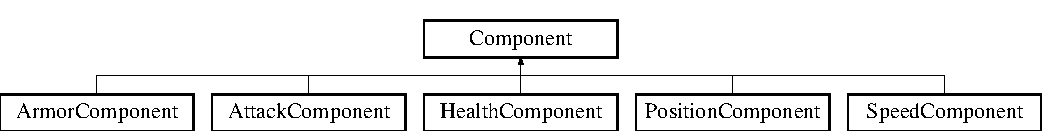
\includegraphics[height=1.763780cm]{structComponent}
\end{center}
\end{figure}
\subsection*{Fonctions membres publiques}
\begin{DoxyCompactItemize}
\item 
virtual void \hyperlink{structComponent_a1d42068fda4a9bf6571810f669b3bb21}{accept} (\hyperlink{classVisitor}{Visitor} \&v)=0
\end{DoxyCompactItemize}


\subsection{Description détaillée}
Classe de base pour les composant. 

une classe de base pour les composant 

\subsection{Documentation des fonctions membres}
\mbox{\Hypertarget{structComponent_a1d42068fda4a9bf6571810f669b3bb21}\label{structComponent_a1d42068fda4a9bf6571810f669b3bb21}} 
\index{Component@{Component}!accept@{accept}}
\index{accept@{accept}!Component@{Component}}
\subsubsection{\texorpdfstring{accept()}{accept()}}
{\footnotesize\ttfamily virtual void Component\+::accept (\begin{DoxyParamCaption}\item[{\hyperlink{classVisitor}{Visitor} \&}]{v }\end{DoxyParamCaption})\hspace{0.3cm}{\ttfamily [pure virtual]}}

Fonction acceptant un visiteur


\begin{DoxyParams}{Paramètres}
{\em V} & le visiteur qui va etre accepter \\
\hline
\end{DoxyParams}


Implémenté dans \hyperlink{structArmorComponent_aac5863d4195fe056fbb0a2a0af17b6e0}{Armor\+Component}, \hyperlink{structAttackComponent_a6644fff9ad3be5bc7cd9571f811fe25e}{Attack\+Component}, \hyperlink{structSpeedComponent_a6857d2108ab631e63a9040bf77a8b366}{Speed\+Component}, \hyperlink{structHealthComponent_a47bb95e02765b03a387366b866046860}{Health\+Component}, et \hyperlink{structPositionComponent_a7f5ef56cf9e5722c7df9fdfa66fdf425}{Position\+Component}.



La documentation de cette structure a été générée à partir du fichier suivant \+:\begin{DoxyCompactItemize}
\item 
include/\hyperlink{Component_8hpp}{Component.\+hpp}\end{DoxyCompactItemize}

\hypertarget{classComponentStorer}{}\section{Référence de la classe Component\+Storer}
\label{classComponentStorer}\index{Component\+Storer@{Component\+Storer}}


{\ttfamily \#include $<$Component\+Storer.\+hpp$>$}

\subsection*{Fonctions membres publiques}
\begin{DoxyCompactItemize}
\item 
{\footnotesize template$<$typename T $>$ }\\std\+::map$<$ int, std\+::shared\+\_\+ptr$<$ \hyperlink{structComponent}{Component} $>$ $>$ \hyperlink{classComponentStorer_abd4fb0cfe30b69e8102e52f66dc35c7a}{get\+Components\+By\+Type} () const
\item 
{\footnotesize template$<$typename T $>$ }\\std\+::shared\+\_\+ptr$<$ \hyperlink{structComponent}{Component} $>$ \hyperlink{classComponentStorer_a817c23e85158ef1fc49592ecd4a02b81}{get\+Component} (int id) const
\item 
std\+::map$<$ std\+::type\+\_\+index, std\+::shared\+\_\+ptr$<$ \hyperlink{structComponent}{Component} $>$ $>$ \hyperlink{classComponentStorer_a32a2e59c11c6d4a73ecec277775225a2}{get\+Components\+By\+Id} (int id) const
\item 
void \hyperlink{classComponentStorer_a563e726b89bb522b40e564cf11f68bda}{add\+Component} (int id, std\+::shared\+\_\+ptr$<$ \hyperlink{structComponent}{Component} $>$ c)
\end{DoxyCompactItemize}


\subsection{Documentation des fonctions membres}
\mbox{\Hypertarget{classComponentStorer_a563e726b89bb522b40e564cf11f68bda}\label{classComponentStorer_a563e726b89bb522b40e564cf11f68bda}} 
\index{Component\+Storer@{Component\+Storer}!add\+Component@{add\+Component}}
\index{add\+Component@{add\+Component}!Component\+Storer@{Component\+Storer}}
\subsubsection{\texorpdfstring{add\+Component()}{addComponent()}}
{\footnotesize\ttfamily void Component\+Storer\+::add\+Component (\begin{DoxyParamCaption}\item[{int}]{id,  }\item[{std\+::shared\+\_\+ptr$<$ \hyperlink{structComponent}{Component} $>$}]{c }\end{DoxyParamCaption})}

\mbox{\Hypertarget{classComponentStorer_a817c23e85158ef1fc49592ecd4a02b81}\label{classComponentStorer_a817c23e85158ef1fc49592ecd4a02b81}} 
\index{Component\+Storer@{Component\+Storer}!get\+Component@{get\+Component}}
\index{get\+Component@{get\+Component}!Component\+Storer@{Component\+Storer}}
\subsubsection{\texorpdfstring{get\+Component()}{getComponent()}}
{\footnotesize\ttfamily template$<$typename T $>$ \\
std\+::shared\+\_\+ptr$<$\hyperlink{structComponent}{Component}$>$ Component\+Storer\+::get\+Component (\begin{DoxyParamCaption}\item[{int}]{id }\end{DoxyParamCaption}) const\hspace{0.3cm}{\ttfamily [inline]}}

\mbox{\Hypertarget{classComponentStorer_a32a2e59c11c6d4a73ecec277775225a2}\label{classComponentStorer_a32a2e59c11c6d4a73ecec277775225a2}} 
\index{Component\+Storer@{Component\+Storer}!get\+Components\+By\+Id@{get\+Components\+By\+Id}}
\index{get\+Components\+By\+Id@{get\+Components\+By\+Id}!Component\+Storer@{Component\+Storer}}
\subsubsection{\texorpdfstring{get\+Components\+By\+Id()}{getComponentsById()}}
{\footnotesize\ttfamily std\+::map$<$ std\+::type\+\_\+index, std\+::shared\+\_\+ptr$<$ \hyperlink{structComponent}{Component} $>$ $>$ Component\+Storer\+::get\+Components\+By\+Id (\begin{DoxyParamCaption}\item[{int}]{id }\end{DoxyParamCaption}) const}

\mbox{\Hypertarget{classComponentStorer_abd4fb0cfe30b69e8102e52f66dc35c7a}\label{classComponentStorer_abd4fb0cfe30b69e8102e52f66dc35c7a}} 
\index{Component\+Storer@{Component\+Storer}!get\+Components\+By\+Type@{get\+Components\+By\+Type}}
\index{get\+Components\+By\+Type@{get\+Components\+By\+Type}!Component\+Storer@{Component\+Storer}}
\subsubsection{\texorpdfstring{get\+Components\+By\+Type()}{getComponentsByType()}}
{\footnotesize\ttfamily template$<$typename T $>$ \\
std\+::map$<$int, std\+::shared\+\_\+ptr$<$\hyperlink{structComponent}{Component}$>$ $>$ Component\+Storer\+::get\+Components\+By\+Type (\begin{DoxyParamCaption}{ }\end{DoxyParamCaption}) const\hspace{0.3cm}{\ttfamily [inline]}}



La documentation de cette classe a été générée à partir des fichiers suivants \+:\begin{DoxyCompactItemize}
\item 
include/\hyperlink{ComponentStorer_8hpp}{Component\+Storer.\+hpp}\item 
src/\hyperlink{ComponentStorer_8cpp}{Component\+Storer.\+cpp}\end{DoxyCompactItemize}

\hypertarget{classEntityCreator}{}\section{Référence de la classe Entity\+Creator}
\label{classEntityCreator}\index{Entity\+Creator@{Entity\+Creator}}


Cette classe a pour but de creer les entites sur demande.  




{\ttfamily \#include $<$Entity\+Creator.\+hpp$>$}

Graphe d\textquotesingle{}héritage de Entity\+Creator\+:\begin{figure}[H]
\begin{center}
\leavevmode
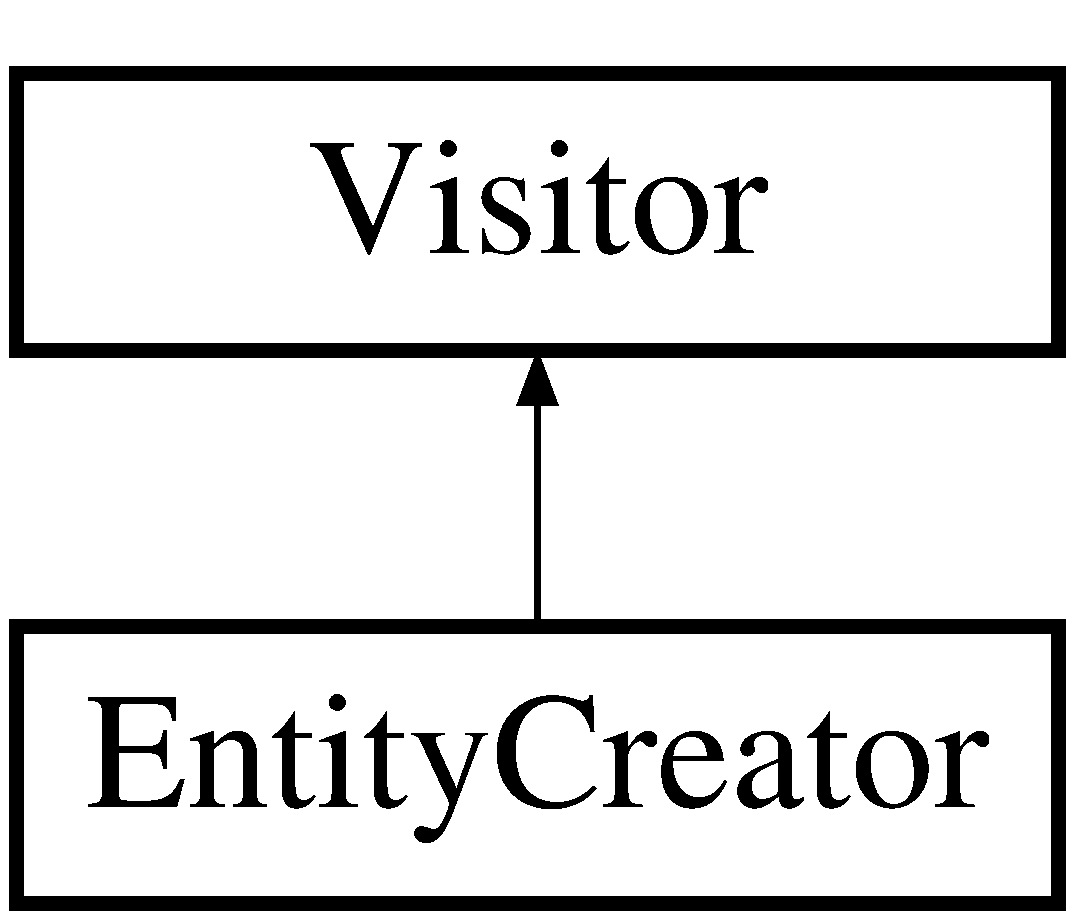
\includegraphics[height=2.000000cm]{classEntityCreator}
\end{center}
\end{figure}
\subsection*{Fonctions membres publiques}
\begin{DoxyCompactItemize}
\item 
\hyperlink{classEntityCreator_acf61fa9cbe29e50bff8a60620e01a3f2}{Entity\+Creator} (\hyperlink{classComponentStorer}{Component\+Storer} \&compS, \hyperlink{classEntityManager}{Entity\+Manager} \&entM, const std\+::string \&script\+Path)
\begin{DoxyCompactList}\small\item\em Constructor. \end{DoxyCompactList}\item 
int \hyperlink{classEntityCreator_a55f031e5e1ea0afc99375bcb0c2ace94}{add\+Entity} (const std\+::string \&ent\+Name)
\item 
void \hyperlink{classEntityCreator_ae6e6fa03f354303f33714c875bda0c62}{visit} (\hyperlink{structPositionComponent}{Position\+Component} \&)
\item 
void \hyperlink{classEntityCreator_aaa96ee2442660da23e34a1f0cec3fa47}{visit} (\hyperlink{structHealthComponent}{Health\+Component} \&)
\item 
void \hyperlink{classEntityCreator_a48a6a070dee113ccf56916c0077845c1}{visit} (\hyperlink{structAttackComponent}{Attack\+Component} \&)
\item 
void \hyperlink{classEntityCreator_af23e7656c8ee20319bd890aad99a6996}{visit} (\hyperlink{structArmorComponent}{Armor\+Component} \&)
\item 
void \hyperlink{classEntityCreator_aee1042f0ec1dc1310ab4c0096d09e094}{visit} (\hyperlink{structSpeedComponent}{Speed\+Component} \&)
\end{DoxyCompactItemize}


\subsection{Description détaillée}
Cette classe a pour but de creer les entites sur demande. 

La classe va charger et stocker des templates de chaque entites et va les copier dans \hyperlink{classComponentStorer}{Component\+Storer} quand on creer l\textquotesingle{}objet 

\subsection{Documentation des constructeurs et destructeur}
\mbox{\Hypertarget{classEntityCreator_acf61fa9cbe29e50bff8a60620e01a3f2}\label{classEntityCreator_acf61fa9cbe29e50bff8a60620e01a3f2}} 
\index{Entity\+Creator@{Entity\+Creator}!Entity\+Creator@{Entity\+Creator}}
\index{Entity\+Creator@{Entity\+Creator}!Entity\+Creator@{Entity\+Creator}}
\subsubsection{\texorpdfstring{Entity\+Creator()}{EntityCreator()}}
{\footnotesize\ttfamily Entity\+Creator\+::\+Entity\+Creator (\begin{DoxyParamCaption}\item[{\hyperlink{classComponentStorer}{Component\+Storer} \&}]{compS,  }\item[{\hyperlink{classEntityManager}{Entity\+Manager} \&}]{entM,  }\item[{const std\+::string \&}]{script\+Path }\end{DoxyParamCaption})}



Constructor. 


\begin{DoxyParams}{Paramètres}
{\em comp\+Storer} & le stockage des composants \\
\hline
{\em ent\+Manager} & le gestionnaire des entites \\
\hline
{\em script\+Path} & le chemin vers le fichier lua contenant les templates des entites \\
\hline
\end{DoxyParams}


\subsection{Documentation des fonctions membres}
\mbox{\Hypertarget{classEntityCreator_a55f031e5e1ea0afc99375bcb0c2ace94}\label{classEntityCreator_a55f031e5e1ea0afc99375bcb0c2ace94}} 
\index{Entity\+Creator@{Entity\+Creator}!add\+Entity@{add\+Entity}}
\index{add\+Entity@{add\+Entity}!Entity\+Creator@{Entity\+Creator}}
\subsubsection{\texorpdfstring{add\+Entity()}{addEntity()}}
{\footnotesize\ttfamily int Entity\+Creator\+::add\+Entity (\begin{DoxyParamCaption}\item[{const std\+::string \&}]{ent\+Name }\end{DoxyParamCaption})}

Cette fonction ajoute une entite dans le gestionnaire et les composant dans le stockage a partir d\textquotesingle{}un template


\begin{DoxyParams}{Paramètres}
{\em ent\+Name} & le nom de l\textquotesingle{}entite a creer \\
\hline
\end{DoxyParams}
\begin{DoxyReturn}{Renvoie}
l\textquotesingle{}id de l\textquotesingle{}entite creer, -\/1 si erreur 
\end{DoxyReturn}
\mbox{\Hypertarget{classEntityCreator_ae6e6fa03f354303f33714c875bda0c62}\label{classEntityCreator_ae6e6fa03f354303f33714c875bda0c62}} 
\index{Entity\+Creator@{Entity\+Creator}!visit@{visit}}
\index{visit@{visit}!Entity\+Creator@{Entity\+Creator}}
\subsubsection{\texorpdfstring{visit()}{visit()}\hspace{0.1cm}{\footnotesize\ttfamily [1/5]}}
{\footnotesize\ttfamily void Entity\+Creator\+::visit (\begin{DoxyParamCaption}\item[{\hyperlink{structPositionComponent}{Position\+Component} \&}]{comp }\end{DoxyParamCaption})\hspace{0.3cm}{\ttfamily [virtual]}}

Permet aux composants de visiter la classe


\begin{DoxyParams}{Paramètres}
{\em comp} & le composant \\
\hline
\end{DoxyParams}


Réimplémentée à partir de \hyperlink{classVisitor_afc865e84cb1293284e6f524a00049b11}{Visitor}.

\mbox{\Hypertarget{classEntityCreator_aaa96ee2442660da23e34a1f0cec3fa47}\label{classEntityCreator_aaa96ee2442660da23e34a1f0cec3fa47}} 
\index{Entity\+Creator@{Entity\+Creator}!visit@{visit}}
\index{visit@{visit}!Entity\+Creator@{Entity\+Creator}}
\subsubsection{\texorpdfstring{visit()}{visit()}\hspace{0.1cm}{\footnotesize\ttfamily [2/5]}}
{\footnotesize\ttfamily void Entity\+Creator\+::visit (\begin{DoxyParamCaption}\item[{\hyperlink{structHealthComponent}{Health\+Component} \&}]{comp }\end{DoxyParamCaption})\hspace{0.3cm}{\ttfamily [virtual]}}

Permet aux composants de visiter la classe


\begin{DoxyParams}{Paramètres}
{\em comp} & le composant \\
\hline
\end{DoxyParams}


Réimplémentée à partir de \hyperlink{classVisitor_aba8f1cab6bd85c2b86ed0b8103d30f45}{Visitor}.

\mbox{\Hypertarget{classEntityCreator_a48a6a070dee113ccf56916c0077845c1}\label{classEntityCreator_a48a6a070dee113ccf56916c0077845c1}} 
\index{Entity\+Creator@{Entity\+Creator}!visit@{visit}}
\index{visit@{visit}!Entity\+Creator@{Entity\+Creator}}
\subsubsection{\texorpdfstring{visit()}{visit()}\hspace{0.1cm}{\footnotesize\ttfamily [3/5]}}
{\footnotesize\ttfamily void Entity\+Creator\+::visit (\begin{DoxyParamCaption}\item[{\hyperlink{structAttackComponent}{Attack\+Component} \&}]{comp }\end{DoxyParamCaption})\hspace{0.3cm}{\ttfamily [virtual]}}

Permet aux composants de visiter la classe


\begin{DoxyParams}{Paramètres}
{\em comp} & le composant \\
\hline
\end{DoxyParams}


Réimplémentée à partir de \hyperlink{classVisitor_a6bcc6c971d8ba324024e3cf8e06e3751}{Visitor}.

\mbox{\Hypertarget{classEntityCreator_af23e7656c8ee20319bd890aad99a6996}\label{classEntityCreator_af23e7656c8ee20319bd890aad99a6996}} 
\index{Entity\+Creator@{Entity\+Creator}!visit@{visit}}
\index{visit@{visit}!Entity\+Creator@{Entity\+Creator}}
\subsubsection{\texorpdfstring{visit()}{visit()}\hspace{0.1cm}{\footnotesize\ttfamily [4/5]}}
{\footnotesize\ttfamily void Entity\+Creator\+::visit (\begin{DoxyParamCaption}\item[{\hyperlink{structArmorComponent}{Armor\+Component} \&}]{comp }\end{DoxyParamCaption})\hspace{0.3cm}{\ttfamily [virtual]}}

Permet aux composants de visiter la classe


\begin{DoxyParams}{Paramètres}
{\em comp} & le composant \\
\hline
\end{DoxyParams}


Réimplémentée à partir de \hyperlink{classVisitor_a05ce14929a5c30d182b46f8843605468}{Visitor}.

\mbox{\Hypertarget{classEntityCreator_aee1042f0ec1dc1310ab4c0096d09e094}\label{classEntityCreator_aee1042f0ec1dc1310ab4c0096d09e094}} 
\index{Entity\+Creator@{Entity\+Creator}!visit@{visit}}
\index{visit@{visit}!Entity\+Creator@{Entity\+Creator}}
\subsubsection{\texorpdfstring{visit()}{visit()}\hspace{0.1cm}{\footnotesize\ttfamily [5/5]}}
{\footnotesize\ttfamily void Entity\+Creator\+::visit (\begin{DoxyParamCaption}\item[{\hyperlink{structSpeedComponent}{Speed\+Component} \&}]{comp }\end{DoxyParamCaption})\hspace{0.3cm}{\ttfamily [virtual]}}

Permet aux composants de visiter la classe


\begin{DoxyParams}{Paramètres}
{\em comp} & le composant \\
\hline
\end{DoxyParams}


Réimplémentée à partir de \hyperlink{classVisitor_a42ce8ce5e7c789dc4b919a088e68829b}{Visitor}.



La documentation de cette classe a été générée à partir des fichiers suivants \+:\begin{DoxyCompactItemize}
\item 
include/\hyperlink{EntityCreator_8hpp}{Entity\+Creator.\+hpp}\item 
src/\hyperlink{EntityCreator_8cpp}{Entity\+Creator.\+cpp}\end{DoxyCompactItemize}

\hypertarget{classEntityManager}{}\section{Référence de la classe Entity\+Manager}
\label{classEntityManager}\index{Entity\+Manager@{Entity\+Manager}}


{\ttfamily \#include $<$Entity\+Manager.\+hpp$>$}

\subsection*{Fonctions membres publiques}
\begin{DoxyCompactItemize}
\item 
unsigned int \hyperlink{classEntityManager_a05b583588490e76e947c5cf8a986b5f7}{get\+Next\+Id} ()
\item 
void \hyperlink{classEntityManager_a2020094cd37ee4d48320c48c030b7053}{remove\+Entity} (unsigned int id)
\item 
std\+::vector$<$ unsigned int $>$ \hyperlink{classEntityManager_a9ea2833e8104a1cc41ba2760148f6d5a}{get\+Entities\+Id} () const
\end{DoxyCompactItemize}


\subsection{Documentation des fonctions membres}
\mbox{\Hypertarget{classEntityManager_a9ea2833e8104a1cc41ba2760148f6d5a}\label{classEntityManager_a9ea2833e8104a1cc41ba2760148f6d5a}} 
\index{Entity\+Manager@{Entity\+Manager}!get\+Entities\+Id@{get\+Entities\+Id}}
\index{get\+Entities\+Id@{get\+Entities\+Id}!Entity\+Manager@{Entity\+Manager}}
\subsubsection{\texorpdfstring{get\+Entities\+Id()}{getEntitiesId()}}
{\footnotesize\ttfamily std\+::vector$<$unsigned int$>$ Entity\+Manager\+::get\+Entities\+Id (\begin{DoxyParamCaption}{ }\end{DoxyParamCaption}) const\hspace{0.3cm}{\ttfamily [inline]}}

\mbox{\Hypertarget{classEntityManager_a05b583588490e76e947c5cf8a986b5f7}\label{classEntityManager_a05b583588490e76e947c5cf8a986b5f7}} 
\index{Entity\+Manager@{Entity\+Manager}!get\+Next\+Id@{get\+Next\+Id}}
\index{get\+Next\+Id@{get\+Next\+Id}!Entity\+Manager@{Entity\+Manager}}
\subsubsection{\texorpdfstring{get\+Next\+Id()}{getNextId()}}
{\footnotesize\ttfamily unsigned int Entity\+Manager\+::get\+Next\+Id (\begin{DoxyParamCaption}{ }\end{DoxyParamCaption})}

\mbox{\Hypertarget{classEntityManager_a2020094cd37ee4d48320c48c030b7053}\label{classEntityManager_a2020094cd37ee4d48320c48c030b7053}} 
\index{Entity\+Manager@{Entity\+Manager}!remove\+Entity@{remove\+Entity}}
\index{remove\+Entity@{remove\+Entity}!Entity\+Manager@{Entity\+Manager}}
\subsubsection{\texorpdfstring{remove\+Entity()}{removeEntity()}}
{\footnotesize\ttfamily void Entity\+Manager\+::remove\+Entity (\begin{DoxyParamCaption}\item[{unsigned int}]{id }\end{DoxyParamCaption})}



La documentation de cette classe a été générée à partir des fichiers suivants \+:\begin{DoxyCompactItemize}
\item 
include/\hyperlink{EntityManager_8hpp}{Entity\+Manager.\+hpp}\item 
src/\hyperlink{EntityManager_8cpp}{Entity\+Manager.\+cpp}\end{DoxyCompactItemize}

\hypertarget{structHealthComponent}{}\section{Référence de la structure Health\+Component}
\label{structHealthComponent}\index{Health\+Component@{Health\+Component}}


{\ttfamily \#include $<$Component.\+hpp$>$}

Graphe d\textquotesingle{}héritage de Health\+Component\+:\begin{figure}[H]
\begin{center}
\leavevmode
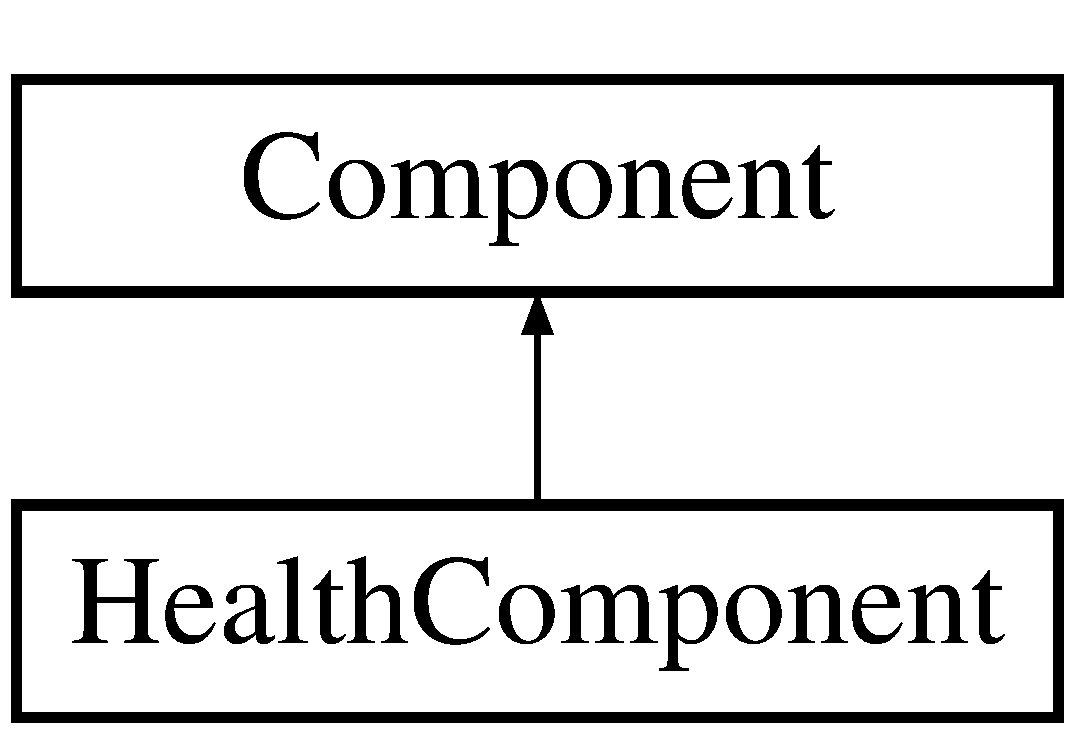
\includegraphics[height=2.000000cm]{structHealthComponent}
\end{center}
\end{figure}
\subsection*{Fonctions membres publiques}
\begin{DoxyCompactItemize}
\item 
\hyperlink{structHealthComponent_aeabc12eec0a3f1ba8f966ce068724d16}{Health\+Component} (int h)
\begin{DoxyCompactList}\small\item\em Constructeur. \end{DoxyCompactList}\item 
virtual void \hyperlink{structHealthComponent_a47bb95e02765b03a387366b866046860}{accept} (\hyperlink{classVisitor}{Visitor} \&v)
\end{DoxyCompactItemize}
\subsection*{Attributs publics}
\begin{DoxyCompactItemize}
\item 
int \hyperlink{structHealthComponent_a44675c84af2972a0cee11b9fff5880b5}{health}
\end{DoxyCompactItemize}


\subsection{Description détaillée}
Composant définissant la vie d\textquotesingle{}une entité 

\subsection{Documentation des constructeurs et destructeur}
\mbox{\Hypertarget{structHealthComponent_aeabc12eec0a3f1ba8f966ce068724d16}\label{structHealthComponent_aeabc12eec0a3f1ba8f966ce068724d16}} 
\index{Health\+Component@{Health\+Component}!Health\+Component@{Health\+Component}}
\index{Health\+Component@{Health\+Component}!Health\+Component@{Health\+Component}}
\subsubsection{\texorpdfstring{Health\+Component()}{HealthComponent()}}
{\footnotesize\ttfamily Health\+Component\+::\+Health\+Component (\begin{DoxyParamCaption}\item[{int}]{h }\end{DoxyParamCaption})\hspace{0.3cm}{\ttfamily [inline]}}



Constructeur. 



\subsection{Documentation des fonctions membres}
\mbox{\Hypertarget{structHealthComponent_a47bb95e02765b03a387366b866046860}\label{structHealthComponent_a47bb95e02765b03a387366b866046860}} 
\index{Health\+Component@{Health\+Component}!accept@{accept}}
\index{accept@{accept}!Health\+Component@{Health\+Component}}
\subsubsection{\texorpdfstring{accept()}{accept()}}
{\footnotesize\ttfamily void Health\+Component\+::accept (\begin{DoxyParamCaption}\item[{\hyperlink{classVisitor}{Visitor} \&}]{v }\end{DoxyParamCaption})\hspace{0.3cm}{\ttfamily [virtual]}}

Fonction acceptant un visiteur


\begin{DoxyParams}{Paramètres}
{\em V} & le visiteur qui va etre accepter \\
\hline
\end{DoxyParams}


Implémente \hyperlink{structComponent_a1d42068fda4a9bf6571810f669b3bb21}{Component}.



\subsection{Documentation des données membres}
\mbox{\Hypertarget{structHealthComponent_a44675c84af2972a0cee11b9fff5880b5}\label{structHealthComponent_a44675c84af2972a0cee11b9fff5880b5}} 
\index{Health\+Component@{Health\+Component}!health@{health}}
\index{health@{health}!Health\+Component@{Health\+Component}}
\subsubsection{\texorpdfstring{health}{health}}
{\footnotesize\ttfamily int Health\+Component\+::health}


\begin{DoxyItemize}
\item la vie de l\textquotesingle{}entite/
\end{DoxyItemize}

/$\ast$$\ast$ Fonction acceptant un visiteur


\begin{DoxyParams}{Paramètres}
{\em V} & le visiteur qui va etre accepter \\
\hline
\end{DoxyParams}


La documentation de cette structure a été générée à partir des fichiers suivants \+:\begin{DoxyCompactItemize}
\item 
include/\hyperlink{Component_8hpp}{Component.\+hpp}\item 
src/\hyperlink{Component_8cpp}{Component.\+cpp}\end{DoxyCompactItemize}

\hypertarget{classLuaScript}{}\section{Référence de la classe Lua\+Script}
\label{classLuaScript}\index{Lua\+Script@{Lua\+Script}}


{\ttfamily \#include $<$Lua\+Script.\+hpp$>$}

\subsection*{Fonctions membres publiques}
\begin{DoxyCompactItemize}
\item 
\hyperlink{classLuaScript_afc0b4a31427c3c78a8529cf3cf6b729e}{Lua\+Script} (const std\+::string \&script\+Name)
\item 
\hyperlink{classLuaScript_a5660ae45ebd4b7a621ae21a2ed0e784b}{$\sim$\+Lua\+Script} ()
\item 
luabridge\+::\+Lua\+Ref \hyperlink{classLuaScript_a7f5b82c910622d8096ece13da5cd85d5}{get} (const std\+::string \&var\+Name)
\item 
std\+::unordered\+\_\+map$<$ std\+::string, luabridge\+::\+Lua\+Ref $>$ \hyperlink{classLuaScript_a05bcad381dac15ea1b5399045651497d}{get\+Key\+Value\+Map} (const luabridge\+::\+Lua\+Ref \&table)
\end{DoxyCompactItemize}


\subsection{Documentation des constructeurs et destructeur}
\mbox{\Hypertarget{classLuaScript_afc0b4a31427c3c78a8529cf3cf6b729e}\label{classLuaScript_afc0b4a31427c3c78a8529cf3cf6b729e}} 
\index{Lua\+Script@{Lua\+Script}!Lua\+Script@{Lua\+Script}}
\index{Lua\+Script@{Lua\+Script}!Lua\+Script@{Lua\+Script}}
\subsubsection{\texorpdfstring{Lua\+Script()}{LuaScript()}}
{\footnotesize\ttfamily Lua\+Script\+::\+Lua\+Script (\begin{DoxyParamCaption}\item[{const std\+::string \&}]{script\+Name }\end{DoxyParamCaption})}

\mbox{\Hypertarget{classLuaScript_a5660ae45ebd4b7a621ae21a2ed0e784b}\label{classLuaScript_a5660ae45ebd4b7a621ae21a2ed0e784b}} 
\index{Lua\+Script@{Lua\+Script}!````~Lua\+Script@{$\sim$\+Lua\+Script}}
\index{````~Lua\+Script@{$\sim$\+Lua\+Script}!Lua\+Script@{Lua\+Script}}
\subsubsection{\texorpdfstring{$\sim$\+Lua\+Script()}{~LuaScript()}}
{\footnotesize\ttfamily Lua\+Script\+::$\sim$\+Lua\+Script (\begin{DoxyParamCaption}{ }\end{DoxyParamCaption})}



\subsection{Documentation des fonctions membres}
\mbox{\Hypertarget{classLuaScript_a7f5b82c910622d8096ece13da5cd85d5}\label{classLuaScript_a7f5b82c910622d8096ece13da5cd85d5}} 
\index{Lua\+Script@{Lua\+Script}!get@{get}}
\index{get@{get}!Lua\+Script@{Lua\+Script}}
\subsubsection{\texorpdfstring{get()}{get()}}
{\footnotesize\ttfamily luabridge\+::\+Lua\+Ref Lua\+Script\+::get (\begin{DoxyParamCaption}\item[{const std\+::string \&}]{var\+Name }\end{DoxyParamCaption})}

\mbox{\Hypertarget{classLuaScript_a05bcad381dac15ea1b5399045651497d}\label{classLuaScript_a05bcad381dac15ea1b5399045651497d}} 
\index{Lua\+Script@{Lua\+Script}!get\+Key\+Value\+Map@{get\+Key\+Value\+Map}}
\index{get\+Key\+Value\+Map@{get\+Key\+Value\+Map}!Lua\+Script@{Lua\+Script}}
\subsubsection{\texorpdfstring{get\+Key\+Value\+Map()}{getKeyValueMap()}}
{\footnotesize\ttfamily std\+::unordered\+\_\+map$<$ std\+::string, luabridge\+::\+Lua\+Ref $>$ Lua\+Script\+::get\+Key\+Value\+Map (\begin{DoxyParamCaption}\item[{const luabridge\+::\+Lua\+Ref \&}]{table }\end{DoxyParamCaption})}



La documentation de cette classe a été générée à partir des fichiers suivants \+:\begin{DoxyCompactItemize}
\item 
include/\hyperlink{LuaScript_8hpp}{Lua\+Script.\+hpp}\item 
src/\hyperlink{LuaScript_8cpp}{Lua\+Script.\+cpp}\end{DoxyCompactItemize}

\hypertarget{classMoveSystem}{}\section{Référence de la classe Move\+System}
\label{classMoveSystem}\index{Move\+System@{Move\+System}}


{\ttfamily \#include $<$Move\+System.\+hpp$>$}

Graphe d\textquotesingle{}héritage de Move\+System\+:\begin{figure}[H]
\begin{center}
\leavevmode
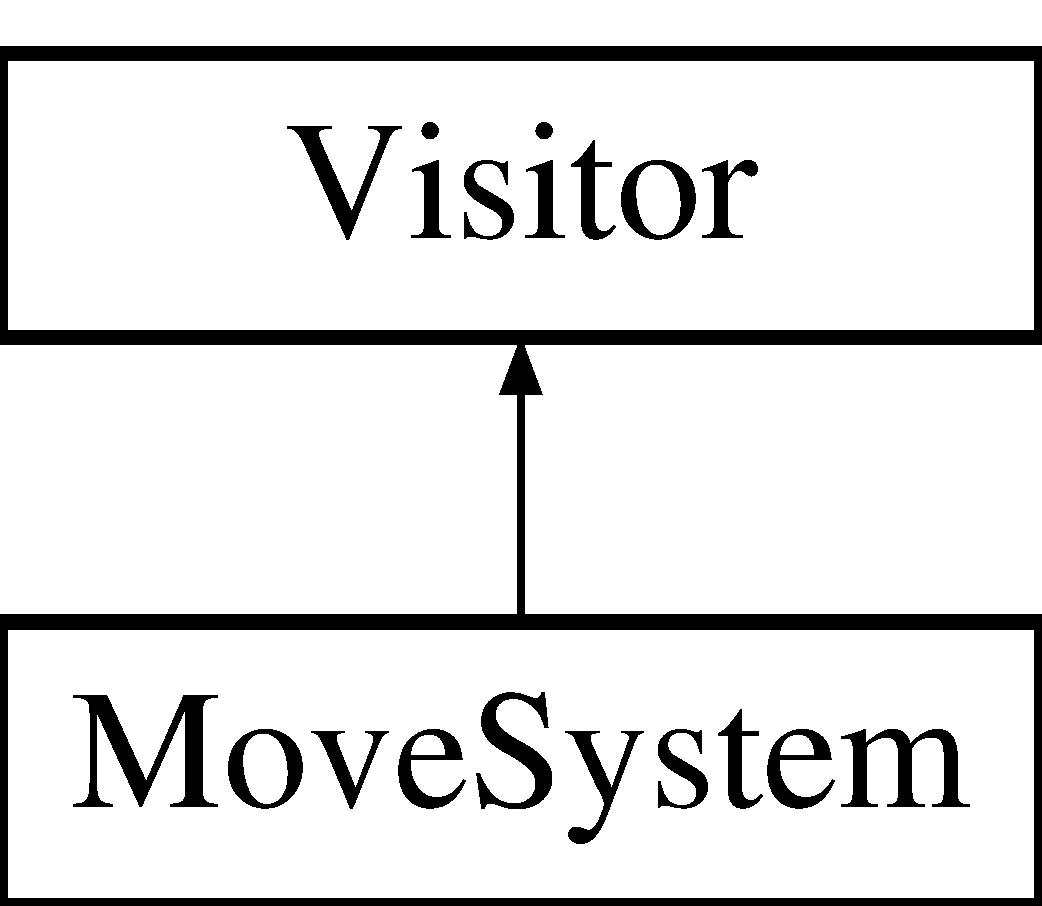
\includegraphics[height=2.000000cm]{classMoveSystem}
\end{center}
\end{figure}
\subsection*{Fonctions membres publiques}
\begin{DoxyCompactItemize}
\item 
\hyperlink{classMoveSystem_a67dc4e8c619b5f28bf73900d1ea2ab9c}{Move\+System} (\hyperlink{classComponentStorer}{Component\+Storer} \&comps, \hyperlink{classEntityManager}{Entity\+Manager} \&entM)
\item 
void \hyperlink{classMoveSystem_ae2ef74a85abacc1f7d4dd02f74620ed2}{update} ()
\item 
void \hyperlink{classMoveSystem_a816baaf8d8d9db45b4c026902946bc1e}{visit} (\hyperlink{structPositionComponent}{Position\+Component} \&p\+Comp)
\end{DoxyCompactItemize}


\subsection{Documentation des constructeurs et destructeur}
\mbox{\Hypertarget{classMoveSystem_a67dc4e8c619b5f28bf73900d1ea2ab9c}\label{classMoveSystem_a67dc4e8c619b5f28bf73900d1ea2ab9c}} 
\index{Move\+System@{Move\+System}!Move\+System@{Move\+System}}
\index{Move\+System@{Move\+System}!Move\+System@{Move\+System}}
\subsubsection{\texorpdfstring{Move\+System()}{MoveSystem()}}
{\footnotesize\ttfamily Move\+System\+::\+Move\+System (\begin{DoxyParamCaption}\item[{\hyperlink{classComponentStorer}{Component\+Storer} \&}]{comps,  }\item[{\hyperlink{classEntityManager}{Entity\+Manager} \&}]{entM }\end{DoxyParamCaption})}



\subsection{Documentation des fonctions membres}
\mbox{\Hypertarget{classMoveSystem_ae2ef74a85abacc1f7d4dd02f74620ed2}\label{classMoveSystem_ae2ef74a85abacc1f7d4dd02f74620ed2}} 
\index{Move\+System@{Move\+System}!update@{update}}
\index{update@{update}!Move\+System@{Move\+System}}
\subsubsection{\texorpdfstring{update()}{update()}}
{\footnotesize\ttfamily void Move\+System\+::update (\begin{DoxyParamCaption}{ }\end{DoxyParamCaption})}

\mbox{\Hypertarget{classMoveSystem_a816baaf8d8d9db45b4c026902946bc1e}\label{classMoveSystem_a816baaf8d8d9db45b4c026902946bc1e}} 
\index{Move\+System@{Move\+System}!visit@{visit}}
\index{visit@{visit}!Move\+System@{Move\+System}}
\subsubsection{\texorpdfstring{visit()}{visit()}}
{\footnotesize\ttfamily void Move\+System\+::visit (\begin{DoxyParamCaption}\item[{\hyperlink{structPositionComponent}{Position\+Component} \&}]{p\+Comp }\end{DoxyParamCaption})\hspace{0.3cm}{\ttfamily [virtual]}}



Réimplémentée à partir de \hyperlink{classVisitor_afc865e84cb1293284e6f524a00049b11}{Visitor}.



La documentation de cette classe a été générée à partir des fichiers suivants \+:\begin{DoxyCompactItemize}
\item 
include/\hyperlink{MoveSystem_8hpp}{Move\+System.\+hpp}\item 
src/\hyperlink{MoveSystem_8cpp}{Move\+System.\+cpp}\end{DoxyCompactItemize}

\hypertarget{structPosition}{}\section{Référence de la structure Position}
\label{structPosition}\index{Position@{Position}}


{\ttfamily \#include $<$Define.\+hpp$>$}

\subsection*{Fonctions membres publiques}
\begin{DoxyCompactItemize}
\item 
\hyperlink{structPosition}{Position} \& \hyperlink{structPosition_ade2e129796afdf1df8769392c2c9aa59}{operator+=} (const \hyperlink{structPosition}{Position} \&r)
\item 
\hyperlink{structPosition}{Position} \& \hyperlink{structPosition_ab665c20a3659543b51ebb671eda086b1}{operator$\ast$=} (int d)
\item 
\hyperlink{structPosition}{Position} \& \hyperlink{structPosition_ae020c1f70717b7e5c4a2202bed3ea0e2}{operator++} ()
\item 
\hyperlink{structPosition}{Position} \hyperlink{structPosition_a512547e3eeacaa34f1b9207d6054d998}{operator++} (int)
\end{DoxyCompactItemize}
\subsection*{Attributs publics}
\begin{DoxyCompactItemize}
\item 
int \hyperlink{structPosition_aeda152ffeee17ae5be9c02327b2408d8}{x}
\item 
int \hyperlink{structPosition_a3c08e9213d4726b21caba3073192c4a3}{y}
\end{DoxyCompactItemize}


\subsection{Documentation des fonctions membres}
\mbox{\Hypertarget{structPosition_ab665c20a3659543b51ebb671eda086b1}\label{structPosition_ab665c20a3659543b51ebb671eda086b1}} 
\index{Position@{Position}!operator$\ast$=@{operator$\ast$=}}
\index{operator$\ast$=@{operator$\ast$=}!Position@{Position}}
\subsubsection{\texorpdfstring{operator$\ast$=()}{operator*=()}}
{\footnotesize\ttfamily \hyperlink{structPosition}{Position} \& Position\+::operator$\ast$= (\begin{DoxyParamCaption}\item[{int}]{d }\end{DoxyParamCaption})}

\mbox{\Hypertarget{structPosition_ae020c1f70717b7e5c4a2202bed3ea0e2}\label{structPosition_ae020c1f70717b7e5c4a2202bed3ea0e2}} 
\index{Position@{Position}!operator++@{operator++}}
\index{operator++@{operator++}!Position@{Position}}
\subsubsection{\texorpdfstring{operator++()}{operator++()}\hspace{0.1cm}{\footnotesize\ttfamily [1/2]}}
{\footnotesize\ttfamily \hyperlink{structPosition}{Position} \& Position\+::operator++ (\begin{DoxyParamCaption}{ }\end{DoxyParamCaption})}

\mbox{\Hypertarget{structPosition_a512547e3eeacaa34f1b9207d6054d998}\label{structPosition_a512547e3eeacaa34f1b9207d6054d998}} 
\index{Position@{Position}!operator++@{operator++}}
\index{operator++@{operator++}!Position@{Position}}
\subsubsection{\texorpdfstring{operator++()}{operator++()}\hspace{0.1cm}{\footnotesize\ttfamily [2/2]}}
{\footnotesize\ttfamily \hyperlink{structPosition}{Position} Position\+::operator++ (\begin{DoxyParamCaption}\item[{int}]{ }\end{DoxyParamCaption})}

\mbox{\Hypertarget{structPosition_ade2e129796afdf1df8769392c2c9aa59}\label{structPosition_ade2e129796afdf1df8769392c2c9aa59}} 
\index{Position@{Position}!operator+=@{operator+=}}
\index{operator+=@{operator+=}!Position@{Position}}
\subsubsection{\texorpdfstring{operator+=()}{operator+=()}}
{\footnotesize\ttfamily \hyperlink{structPosition}{Position} \& Position\+::operator+= (\begin{DoxyParamCaption}\item[{const \hyperlink{structPosition}{Position} \&}]{r }\end{DoxyParamCaption})}



\subsection{Documentation des données membres}
\mbox{\Hypertarget{structPosition_aeda152ffeee17ae5be9c02327b2408d8}\label{structPosition_aeda152ffeee17ae5be9c02327b2408d8}} 
\index{Position@{Position}!x@{x}}
\index{x@{x}!Position@{Position}}
\subsubsection{\texorpdfstring{x}{x}}
{\footnotesize\ttfamily int Position\+::x}

\mbox{\Hypertarget{structPosition_a3c08e9213d4726b21caba3073192c4a3}\label{structPosition_a3c08e9213d4726b21caba3073192c4a3}} 
\index{Position@{Position}!y@{y}}
\index{y@{y}!Position@{Position}}
\subsubsection{\texorpdfstring{y}{y}}
{\footnotesize\ttfamily int Position\+::y}



La documentation de cette structure a été générée à partir des fichiers suivants \+:\begin{DoxyCompactItemize}
\item 
include/\hyperlink{Define_8hpp}{Define.\+hpp}\item 
src/\hyperlink{Define_8cpp}{Define.\+cpp}\end{DoxyCompactItemize}

\hypertarget{structPositionComponent}{}\section{Référence de la structure Position\+Component}
\label{structPositionComponent}\index{Position\+Component@{Position\+Component}}


{\ttfamily \#include $<$Component.\+hpp$>$}

Graphe d\textquotesingle{}héritage de Position\+Component\+:\begin{figure}[H]
\begin{center}
\leavevmode
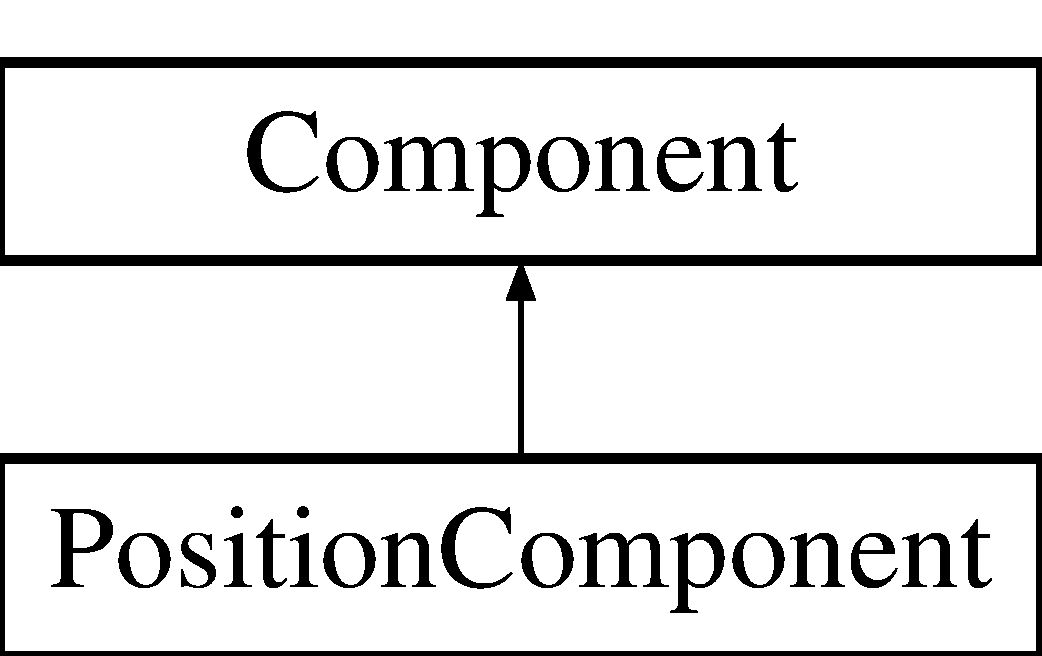
\includegraphics[height=2.000000cm]{structPositionComponent}
\end{center}
\end{figure}
\subsection*{Fonctions membres publiques}
\begin{DoxyCompactItemize}
\item 
\hyperlink{structPositionComponent_af8c7fde08522e4ad2c911a9759ce1808}{Position\+Component} (\hyperlink{structPosition}{Position} p)
\begin{DoxyCompactList}\small\item\em Constructeur. \end{DoxyCompactList}\item 
virtual void \hyperlink{structPositionComponent_a7f5ef56cf9e5722c7df9fdfa66fdf425}{accept} (\hyperlink{classVisitor}{Visitor} \&v)
\end{DoxyCompactItemize}
\subsection*{Attributs publics}
\begin{DoxyCompactItemize}
\item 
\hyperlink{structPosition}{Position} \hyperlink{structPositionComponent_a7fa8d03108cdb0645f12016ba8cd59c9}{position}
\end{DoxyCompactItemize}


\subsection{Description détaillée}
Composant définissant la position d\textquotesingle{}une entite 

\subsection{Documentation des constructeurs et destructeur}
\mbox{\Hypertarget{structPositionComponent_af8c7fde08522e4ad2c911a9759ce1808}\label{structPositionComponent_af8c7fde08522e4ad2c911a9759ce1808}} 
\index{Position\+Component@{Position\+Component}!Position\+Component@{Position\+Component}}
\index{Position\+Component@{Position\+Component}!Position\+Component@{Position\+Component}}
\subsubsection{\texorpdfstring{Position\+Component()}{PositionComponent()}}
{\footnotesize\ttfamily Position\+Component\+::\+Position\+Component (\begin{DoxyParamCaption}\item[{\hyperlink{structPosition}{Position}}]{p }\end{DoxyParamCaption})\hspace{0.3cm}{\ttfamily [inline]}}



Constructeur. 



\subsection{Documentation des fonctions membres}
\mbox{\Hypertarget{structPositionComponent_a7f5ef56cf9e5722c7df9fdfa66fdf425}\label{structPositionComponent_a7f5ef56cf9e5722c7df9fdfa66fdf425}} 
\index{Position\+Component@{Position\+Component}!accept@{accept}}
\index{accept@{accept}!Position\+Component@{Position\+Component}}
\subsubsection{\texorpdfstring{accept()}{accept()}}
{\footnotesize\ttfamily void Position\+Component\+::accept (\begin{DoxyParamCaption}\item[{\hyperlink{classVisitor}{Visitor} \&}]{v }\end{DoxyParamCaption})\hspace{0.3cm}{\ttfamily [virtual]}}

Fonction acceptant un visiteur


\begin{DoxyParams}{Paramètres}
{\em V} & le visiteur qui va etre accepter \\
\hline
\end{DoxyParams}


Implémente \hyperlink{structComponent_a1d42068fda4a9bf6571810f669b3bb21}{Component}.



\subsection{Documentation des données membres}
\mbox{\Hypertarget{structPositionComponent_a7fa8d03108cdb0645f12016ba8cd59c9}\label{structPositionComponent_a7fa8d03108cdb0645f12016ba8cd59c9}} 
\index{Position\+Component@{Position\+Component}!position@{position}}
\index{position@{position}!Position\+Component@{Position\+Component}}
\subsubsection{\texorpdfstring{position}{position}}
{\footnotesize\ttfamily \hyperlink{structPosition}{Position} Position\+Component\+::position}

la position de l\textquotesingle{}entité 

La documentation de cette structure a été générée à partir des fichiers suivants \+:\begin{DoxyCompactItemize}
\item 
include/\hyperlink{Component_8hpp}{Component.\+hpp}\item 
src/\hyperlink{Component_8cpp}{Component.\+cpp}\end{DoxyCompactItemize}

\hypertarget{structSpeedComponent}{}\section{Référence de la structure Speed\+Component}
\label{structSpeedComponent}\index{Speed\+Component@{Speed\+Component}}


{\ttfamily \#include $<$Component.\+hpp$>$}

Graphe d\textquotesingle{}héritage de Speed\+Component\+:\begin{figure}[H]
\begin{center}
\leavevmode
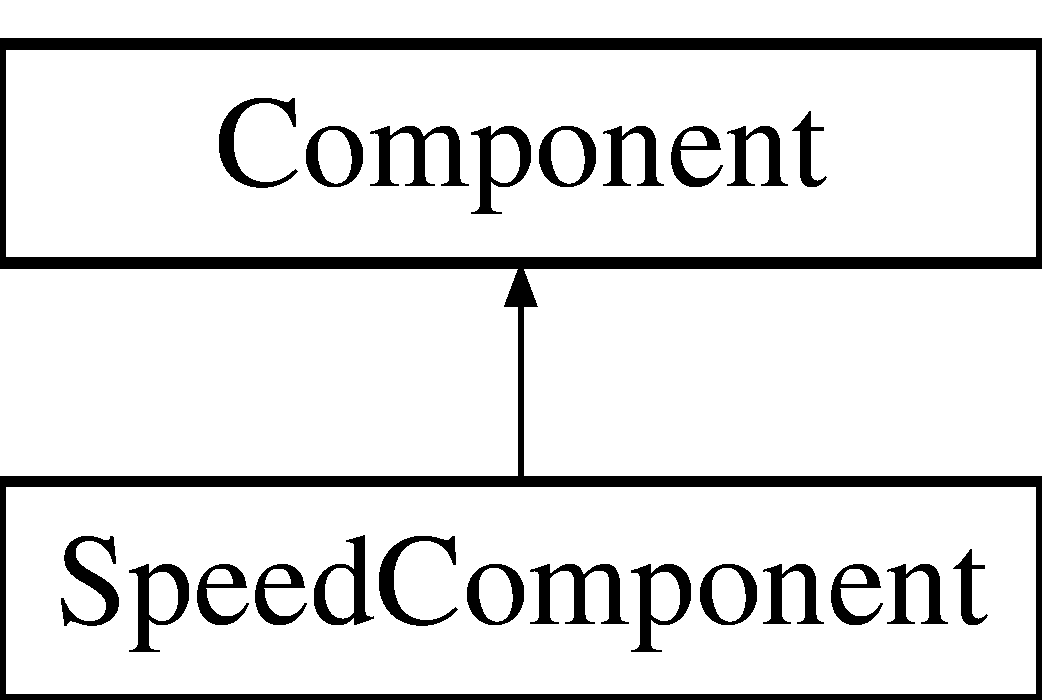
\includegraphics[height=2.000000cm]{structSpeedComponent}
\end{center}
\end{figure}
\subsection*{Fonctions membres publiques}
\begin{DoxyCompactItemize}
\item 
\hyperlink{structSpeedComponent_ac1fd46b8ddbb87e266d8813d9ed82145}{Speed\+Component} (int s)
\item 
virtual void \hyperlink{structSpeedComponent_a6857d2108ab631e63a9040bf77a8b366}{accept} (\hyperlink{classVisitor}{Visitor} \&v)
\end{DoxyCompactItemize}
\subsection*{Attributs publics}
\begin{DoxyCompactItemize}
\item 
int \hyperlink{structSpeedComponent_aedd25677bc7888cab4eac92c444e0cdb}{speed}
\end{DoxyCompactItemize}


\subsection{Documentation des constructeurs et destructeur}
\mbox{\Hypertarget{structSpeedComponent_ac1fd46b8ddbb87e266d8813d9ed82145}\label{structSpeedComponent_ac1fd46b8ddbb87e266d8813d9ed82145}} 
\index{Speed\+Component@{Speed\+Component}!Speed\+Component@{Speed\+Component}}
\index{Speed\+Component@{Speed\+Component}!Speed\+Component@{Speed\+Component}}
\subsubsection{\texorpdfstring{Speed\+Component()}{SpeedComponent()}}
{\footnotesize\ttfamily Speed\+Component\+::\+Speed\+Component (\begin{DoxyParamCaption}\item[{int}]{s }\end{DoxyParamCaption})\hspace{0.3cm}{\ttfamily [inline]}}



\subsection{Documentation des fonctions membres}
\mbox{\Hypertarget{structSpeedComponent_a6857d2108ab631e63a9040bf77a8b366}\label{structSpeedComponent_a6857d2108ab631e63a9040bf77a8b366}} 
\index{Speed\+Component@{Speed\+Component}!accept@{accept}}
\index{accept@{accept}!Speed\+Component@{Speed\+Component}}
\subsubsection{\texorpdfstring{accept()}{accept()}}
{\footnotesize\ttfamily void Speed\+Component\+::accept (\begin{DoxyParamCaption}\item[{\hyperlink{classVisitor}{Visitor} \&}]{v }\end{DoxyParamCaption})\hspace{0.3cm}{\ttfamily [virtual]}}

Fonction acceptant un visiteur


\begin{DoxyParams}{Paramètres}
{\em V} & le visiteur qui va etre accepter \\
\hline
\end{DoxyParams}


Implémente \hyperlink{structComponent_a1d42068fda4a9bf6571810f669b3bb21}{Component}.



\subsection{Documentation des données membres}
\mbox{\Hypertarget{structSpeedComponent_aedd25677bc7888cab4eac92c444e0cdb}\label{structSpeedComponent_aedd25677bc7888cab4eac92c444e0cdb}} 
\index{Speed\+Component@{Speed\+Component}!speed@{speed}}
\index{speed@{speed}!Speed\+Component@{Speed\+Component}}
\subsubsection{\texorpdfstring{speed}{speed}}
{\footnotesize\ttfamily int Speed\+Component\+::speed}



La documentation de cette structure a été générée à partir des fichiers suivants \+:\begin{DoxyCompactItemize}
\item 
include/\hyperlink{Component_8hpp}{Component.\+hpp}\item 
src/\hyperlink{Component_8cpp}{Component.\+cpp}\end{DoxyCompactItemize}

\hypertarget{classVisitor}{}\section{Référence de la classe Visitor}
\label{classVisitor}\index{Visitor@{Visitor}}


{\ttfamily \#include $<$Component.\+hpp$>$}

Graphe d\textquotesingle{}héritage de Visitor\+:\begin{figure}[H]
\begin{center}
\leavevmode
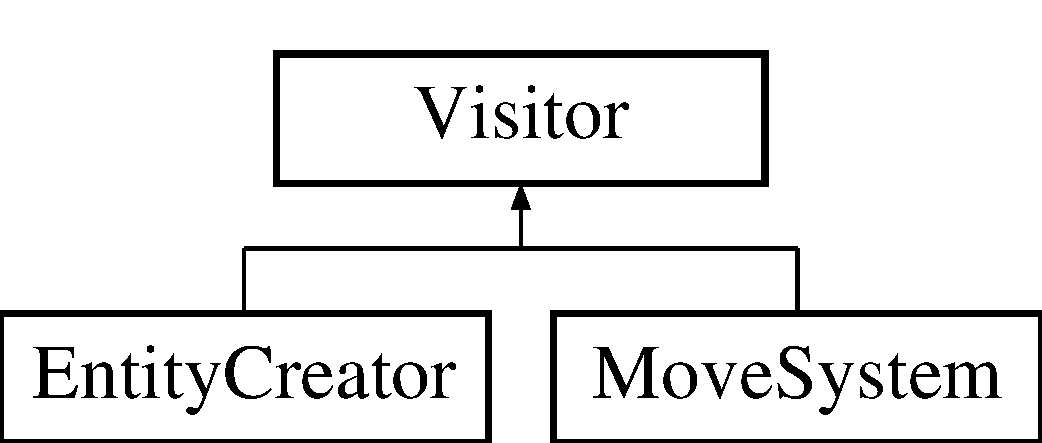
\includegraphics[height=2.000000cm]{classVisitor}
\end{center}
\end{figure}
\subsection*{Fonctions membres publiques}
\begin{DoxyCompactItemize}
\item 
virtual \hyperlink{classVisitor_a02ffa1442ae77b4dbc1dc362be511dc5}{$\sim$\+Visitor} ()=0
\item 
virtual void \hyperlink{classVisitor_afc865e84cb1293284e6f524a00049b11}{visit} (\hyperlink{structPositionComponent}{Position\+Component} \&comp)
\item 
virtual void \hyperlink{classVisitor_aba8f1cab6bd85c2b86ed0b8103d30f45}{visit} (\hyperlink{structHealthComponent}{Health\+Component} \&comp)
\item 
virtual void \hyperlink{classVisitor_a6bcc6c971d8ba324024e3cf8e06e3751}{visit} (\hyperlink{structAttackComponent}{Attack\+Component} \&comp)
\item 
virtual void \hyperlink{classVisitor_a05ce14929a5c30d182b46f8843605468}{visit} (\hyperlink{structArmorComponent}{Armor\+Component} \&comp)
\item 
virtual void \hyperlink{classVisitor_a42ce8ce5e7c789dc4b919a088e68829b}{visit} (\hyperlink{structSpeedComponent}{Speed\+Component} \&comp)
\end{DoxyCompactItemize}


\subsection{Documentation des constructeurs et destructeur}
\mbox{\Hypertarget{classVisitor_a02ffa1442ae77b4dbc1dc362be511dc5}\label{classVisitor_a02ffa1442ae77b4dbc1dc362be511dc5}} 
\index{Visitor@{Visitor}!````~Visitor@{$\sim$\+Visitor}}
\index{````~Visitor@{$\sim$\+Visitor}!Visitor@{Visitor}}
\subsubsection{\texorpdfstring{$\sim$\+Visitor()}{~Visitor()}}
{\footnotesize\ttfamily Visitor\+::$\sim$\+Visitor (\begin{DoxyParamCaption}{ }\end{DoxyParamCaption})\hspace{0.3cm}{\ttfamily [inline]}, {\ttfamily [pure virtual]}}



\subsection{Documentation des fonctions membres}
\mbox{\Hypertarget{classVisitor_afc865e84cb1293284e6f524a00049b11}\label{classVisitor_afc865e84cb1293284e6f524a00049b11}} 
\index{Visitor@{Visitor}!visit@{visit}}
\index{visit@{visit}!Visitor@{Visitor}}
\subsubsection{\texorpdfstring{visit()}{visit()}\hspace{0.1cm}{\footnotesize\ttfamily [1/5]}}
{\footnotesize\ttfamily virtual void Visitor\+::visit (\begin{DoxyParamCaption}\item[{\hyperlink{structPositionComponent}{Position\+Component} \&}]{comp }\end{DoxyParamCaption})\hspace{0.3cm}{\ttfamily [inline]}, {\ttfamily [virtual]}}



Réimplémentée dans \hyperlink{classEntityCreator_ae6e6fa03f354303f33714c875bda0c62}{Entity\+Creator}, et \hyperlink{classMoveSystem_a816baaf8d8d9db45b4c026902946bc1e}{Move\+System}.

\mbox{\Hypertarget{classVisitor_aba8f1cab6bd85c2b86ed0b8103d30f45}\label{classVisitor_aba8f1cab6bd85c2b86ed0b8103d30f45}} 
\index{Visitor@{Visitor}!visit@{visit}}
\index{visit@{visit}!Visitor@{Visitor}}
\subsubsection{\texorpdfstring{visit()}{visit()}\hspace{0.1cm}{\footnotesize\ttfamily [2/5]}}
{\footnotesize\ttfamily virtual void Visitor\+::visit (\begin{DoxyParamCaption}\item[{\hyperlink{structHealthComponent}{Health\+Component} \&}]{comp }\end{DoxyParamCaption})\hspace{0.3cm}{\ttfamily [inline]}, {\ttfamily [virtual]}}



Réimplémentée dans \hyperlink{classEntityCreator_aaa96ee2442660da23e34a1f0cec3fa47}{Entity\+Creator}.

\mbox{\Hypertarget{classVisitor_a6bcc6c971d8ba324024e3cf8e06e3751}\label{classVisitor_a6bcc6c971d8ba324024e3cf8e06e3751}} 
\index{Visitor@{Visitor}!visit@{visit}}
\index{visit@{visit}!Visitor@{Visitor}}
\subsubsection{\texorpdfstring{visit()}{visit()}\hspace{0.1cm}{\footnotesize\ttfamily [3/5]}}
{\footnotesize\ttfamily virtual void Visitor\+::visit (\begin{DoxyParamCaption}\item[{\hyperlink{structAttackComponent}{Attack\+Component} \&}]{comp }\end{DoxyParamCaption})\hspace{0.3cm}{\ttfamily [inline]}, {\ttfamily [virtual]}}



Réimplémentée dans \hyperlink{classEntityCreator_a48a6a070dee113ccf56916c0077845c1}{Entity\+Creator}.

\mbox{\Hypertarget{classVisitor_a05ce14929a5c30d182b46f8843605468}\label{classVisitor_a05ce14929a5c30d182b46f8843605468}} 
\index{Visitor@{Visitor}!visit@{visit}}
\index{visit@{visit}!Visitor@{Visitor}}
\subsubsection{\texorpdfstring{visit()}{visit()}\hspace{0.1cm}{\footnotesize\ttfamily [4/5]}}
{\footnotesize\ttfamily virtual void Visitor\+::visit (\begin{DoxyParamCaption}\item[{\hyperlink{structArmorComponent}{Armor\+Component} \&}]{comp }\end{DoxyParamCaption})\hspace{0.3cm}{\ttfamily [inline]}, {\ttfamily [virtual]}}



Réimplémentée dans \hyperlink{classEntityCreator_af23e7656c8ee20319bd890aad99a6996}{Entity\+Creator}.

\mbox{\Hypertarget{classVisitor_a42ce8ce5e7c789dc4b919a088e68829b}\label{classVisitor_a42ce8ce5e7c789dc4b919a088e68829b}} 
\index{Visitor@{Visitor}!visit@{visit}}
\index{visit@{visit}!Visitor@{Visitor}}
\subsubsection{\texorpdfstring{visit()}{visit()}\hspace{0.1cm}{\footnotesize\ttfamily [5/5]}}
{\footnotesize\ttfamily virtual void Visitor\+::visit (\begin{DoxyParamCaption}\item[{\hyperlink{structSpeedComponent}{Speed\+Component} \&}]{comp }\end{DoxyParamCaption})\hspace{0.3cm}{\ttfamily [inline]}, {\ttfamily [virtual]}}



Réimplémentée dans \hyperlink{classEntityCreator_aee1042f0ec1dc1310ab4c0096d09e094}{Entity\+Creator}.



La documentation de cette classe a été générée à partir du fichier suivant \+:\begin{DoxyCompactItemize}
\item 
include/\hyperlink{Component_8hpp}{Component.\+hpp}\end{DoxyCompactItemize}

\chapter{Documentation des fichiers}
\hypertarget{Component_8hpp}{}\section{Référence du fichier include/\+Component.hpp}
\label{Component_8hpp}\index{include/\+Component.\+hpp@{include/\+Component.\+hpp}}


Ici sont declares les class \hyperlink{classVisitor}{Visitor}, \hyperlink{structComponent}{Component} et les class filles de component.  


{\ttfamily \#include \char`\"{}Define.\+hpp\char`\"{}}\newline
{\ttfamily \#include $<$S\+F\+M\+L/\+Graphics.\+hpp$>$}\newline
{\ttfamily \#include $<$array$>$}\newline
{\ttfamily \#include $<$memory$>$}\newline
\subsection*{Classes}
\begin{DoxyCompactItemize}
\item 
struct \hyperlink{structComponent}{Component}
\begin{DoxyCompactList}\small\item\em Classe de base pour les composant. \end{DoxyCompactList}\item 
struct \hyperlink{structPositionComponent}{Position\+Component}
\item 
struct \hyperlink{structHealthComponent}{Health\+Component}
\item 
struct \hyperlink{structSpeedComponent}{Speed\+Component}
\item 
struct \hyperlink{structAttackComponent}{Attack\+Component}
\item 
struct \hyperlink{structArmorComponent}{Armor\+Component}
\item 
class \hyperlink{classVisitor}{Visitor}
\end{DoxyCompactItemize}


\subsection{Description détaillée}
Ici sont declares les class \hyperlink{classVisitor}{Visitor}, \hyperlink{structComponent}{Component} et les class filles de component. 

\begin{DoxyAuthor}{Auteur}
Papy\+Redstone 
\end{DoxyAuthor}
\begin{DoxyVersion}{Version}
1.\+0 
\end{DoxyVersion}

\hypertarget{ComponentStorer_8hpp}{}\section{Référence du fichier include/\+Component\+Storer.hpp}
\label{ComponentStorer_8hpp}\index{include/\+Component\+Storer.\+hpp@{include/\+Component\+Storer.\+hpp}}
{\ttfamily \#include \char`\"{}Component.\+hpp\char`\"{}}\newline
{\ttfamily \#include $<$memory$>$}\newline
{\ttfamily \#include $<$map$>$}\newline
{\ttfamily \#include $<$vector$>$}\newline
{\ttfamily \#include $<$typeindex$>$}\newline
{\ttfamily \#include $<$iostream$>$}\newline
\subsection*{Classes}
\begin{DoxyCompactItemize}
\item 
class \hyperlink{classComponentStorer}{Component\+Storer}
\end{DoxyCompactItemize}

\hypertarget{Define_8hpp}{}\section{Référence du fichier include/\+Define.hpp}
\label{Define_8hpp}\index{include/\+Define.\+hpp@{include/\+Define.\+hpp}}
{\ttfamily \#include $<$array$>$}\newline
\subsection*{Classes}
\begin{DoxyCompactItemize}
\item 
struct \hyperlink{structPosition}{Position}
\end{DoxyCompactItemize}
\subsection*{Espaces de nommage}
\begin{DoxyCompactItemize}
\item 
 \hyperlink{namespaceDommageType}{Dommage\+Type}
\item 
 \hyperlink{namespaceAttackType}{Attack\+Type}
\item 
 \hyperlink{namespaceDirection}{Direction}
\end{DoxyCompactItemize}
\subsection*{Énumérations}
\begin{DoxyCompactItemize}
\item 
enum \hyperlink{namespaceDommageType_a6e5dff665b7631fe6ec9065dddbebcfd}{Dommage\+Type\+::\+Type} \{ \hyperlink{namespaceDommageType_a6e5dff665b7631fe6ec9065dddbebcfdabca33f1e8d86b9faddd26010eb172ec0}{Dommage\+Type\+::\+Pierce}, 
\hyperlink{namespaceDommageType_a6e5dff665b7631fe6ec9065dddbebcfdad7195516d2e659e73c0f22e64249517b}{Dommage\+Type\+::\+Shock}, 
\hyperlink{namespaceDommageType_a6e5dff665b7631fe6ec9065dddbebcfdab12cf1b0c6c2cd00d9466c6cab208137}{Dommage\+Type\+::\+Magic}, 
\hyperlink{namespaceDommageType_a6e5dff665b7631fe6ec9065dddbebcfda11352066c669cc04a816c1fbc404eb5f}{Dommage\+Type\+::\+N\+O\+NE}
 \}
\item 
enum \hyperlink{namespaceAttackType_a26a2d73c5f73a06a63a568dcd519d302}{Attack\+Type\+::\+Type} \{ \hyperlink{namespaceAttackType_a26a2d73c5f73a06a63a568dcd519d302a53add169c04afbf920774a3cdf710106}{Attack\+Type\+::\+Melee}, 
\hyperlink{namespaceAttackType_a26a2d73c5f73a06a63a568dcd519d302a3a9ed6c6d45ca13d8df01c12f7d538fd}{Attack\+Type\+::\+Distance}, 
\hyperlink{namespaceAttackType_a26a2d73c5f73a06a63a568dcd519d302a73b8be32d0bc40ff4a231436e331f161}{Attack\+Type\+::\+N\+O\+NE}
 \}
\item 
enum \hyperlink{namespaceDirection_aaa56ca1cc2883e1cab31b6cbb5054418}{Direction\+::\+Dir} \{ \newline
\hyperlink{namespaceDirection_aaa56ca1cc2883e1cab31b6cbb5054418a2dcf8e71283b05e59e3b7d1fa4228623}{Direction\+::\+Up}, 
\hyperlink{namespaceDirection_aaa56ca1cc2883e1cab31b6cbb5054418aad5dbfe9b746123d7af7381b52a183f1}{Direction\+::\+Down}, 
\hyperlink{namespaceDirection_aaa56ca1cc2883e1cab31b6cbb5054418aa6314d583c5d1432de99eb3fda30bdea}{Direction\+::\+Left}, 
\hyperlink{namespaceDirection_aaa56ca1cc2883e1cab31b6cbb5054418a1d010c1da83b45aa3ded2cb937d2d979}{Direction\+::\+Right}, 
\newline
\hyperlink{namespaceDirection_aaa56ca1cc2883e1cab31b6cbb5054418a1f9c924b3a1502e5e35ed148994c4148}{Direction\+::\+None}
 \}
\end{DoxyCompactItemize}
\subsection*{Fonctions}
\begin{DoxyCompactItemize}
\item 
bool \hyperlink{Define_8hpp_a1b4ef906d1f4cbcc1acbdf35518b6081}{operator==} (const \hyperlink{structPosition}{Position} \&l, const \hyperlink{structPosition}{Position} \&r)
\item 
\hyperlink{structPosition}{Position} \hyperlink{Define_8hpp_aebe6095cc1b978b08daff33822be6e8e}{operator+} (const \hyperlink{structPosition}{Position} \&l, const \hyperlink{structPosition}{Position} \&r)
\item 
\hyperlink{structPosition}{Position} \hyperlink{Define_8hpp_ab14a51b3479d56b3901395ee1d9ec36d}{operator$\ast$} (const \hyperlink{structPosition}{Position} \&l, int d)
\end{DoxyCompactItemize}
\subsection*{Variables}
\begin{DoxyCompactItemize}
\item 
const std\+::array$<$ Type, 3 $>$ \hyperlink{namespaceDommageType_a95378d0bf91b2850a1a5c112c35bb75c}{Dommage\+Type\+::\+All} = \{Shock, Pierce, Magic\}
\item 
const std\+::array$<$ Type, 2 $>$ \hyperlink{namespaceAttackType_a44c88a70d0a57861180381c34bda18e9}{Attack\+Type\+::\+All} = \{Melee, Distance\}
\item 
const std\+::array$<$ Dir, 4 $>$ \hyperlink{namespaceDirection_aabd5fd5d609f7dda7f8f50f1dbd563a7}{Direction\+::\+All} = \{Up, Down, Left, Right\}
\end{DoxyCompactItemize}


\subsection{Documentation des fonctions}
\mbox{\Hypertarget{Define_8hpp_ab14a51b3479d56b3901395ee1d9ec36d}\label{Define_8hpp_ab14a51b3479d56b3901395ee1d9ec36d}} 
\index{Define.\+hpp@{Define.\+hpp}!operator$\ast$@{operator$\ast$}}
\index{operator$\ast$@{operator$\ast$}!Define.\+hpp@{Define.\+hpp}}
\subsubsection{\texorpdfstring{operator$\ast$()}{operator*()}}
{\footnotesize\ttfamily \hyperlink{structPosition}{Position} operator$\ast$ (\begin{DoxyParamCaption}\item[{const \hyperlink{structPosition}{Position} \&}]{l,  }\item[{int}]{d }\end{DoxyParamCaption})}

\mbox{\Hypertarget{Define_8hpp_aebe6095cc1b978b08daff33822be6e8e}\label{Define_8hpp_aebe6095cc1b978b08daff33822be6e8e}} 
\index{Define.\+hpp@{Define.\+hpp}!operator+@{operator+}}
\index{operator+@{operator+}!Define.\+hpp@{Define.\+hpp}}
\subsubsection{\texorpdfstring{operator+()}{operator+()}}
{\footnotesize\ttfamily \hyperlink{structPosition}{Position} operator+ (\begin{DoxyParamCaption}\item[{const \hyperlink{structPosition}{Position} \&}]{l,  }\item[{const \hyperlink{structPosition}{Position} \&}]{r }\end{DoxyParamCaption})}

\mbox{\Hypertarget{Define_8hpp_a1b4ef906d1f4cbcc1acbdf35518b6081}\label{Define_8hpp_a1b4ef906d1f4cbcc1acbdf35518b6081}} 
\index{Define.\+hpp@{Define.\+hpp}!operator==@{operator==}}
\index{operator==@{operator==}!Define.\+hpp@{Define.\+hpp}}
\subsubsection{\texorpdfstring{operator==()}{operator==()}}
{\footnotesize\ttfamily bool operator== (\begin{DoxyParamCaption}\item[{const \hyperlink{structPosition}{Position} \&}]{l,  }\item[{const \hyperlink{structPosition}{Position} \&}]{r }\end{DoxyParamCaption})}


\hypertarget{ECS_8hpp}{}\section{Référence du fichier include/\+E\+CS.hpp}
\label{ECS_8hpp}\index{include/\+E\+C\+S.\+hpp@{include/\+E\+C\+S.\+hpp}}
{\ttfamily \#include \char`\"{}Move\+System.\+hpp\char`\"{}}\newline

\hypertarget{ECSEntity_8hpp}{}\section{Référence du fichier include/\+E\+C\+S\+Entity.hpp}
\label{ECSEntity_8hpp}\index{include/\+E\+C\+S\+Entity.\+hpp@{include/\+E\+C\+S\+Entity.\+hpp}}
{\ttfamily \#include \char`\"{}Component.\+hpp\char`\"{}}\newline
{\ttfamily \#include \char`\"{}Component\+Storer.\+hpp\char`\"{}}\newline
{\ttfamily \#include \char`\"{}Entity\+Manager.\+hpp\char`\"{}}\newline
{\ttfamily \#include \char`\"{}Entity\+Creator.\+hpp\char`\"{}}\newline

\hypertarget{EntityCreator_8hpp}{}\section{Référence du fichier include/\+Entity\+Creator.hpp}
\label{EntityCreator_8hpp}\index{include/\+Entity\+Creator.\+hpp@{include/\+Entity\+Creator.\+hpp}}


Ici est declare la class \hyperlink{classEntityCreator}{Entity\+Creator}.  


{\ttfamily \#include \char`\"{}Component\+Storer.\+hpp\char`\"{}}\newline
{\ttfamily \#include \char`\"{}Entity\+Manager.\+hpp\char`\"{}}\newline
{\ttfamily \#include \char`\"{}Lua\+Script.\+hpp\char`\"{}}\newline
{\ttfamily \#include $<$map$>$}\newline
{\ttfamily \#include $<$memory$>$}\newline
{\ttfamily \#include $<$string$>$}\newline
{\ttfamily \#include $<$vector$>$}\newline
{\ttfamily \#include $<$cassert$>$}\newline
\subsection*{Classes}
\begin{DoxyCompactItemize}
\item 
class \hyperlink{classEntityCreator}{Entity\+Creator}
\begin{DoxyCompactList}\small\item\em Cette classe a pour but de creer les entites sur demande. \end{DoxyCompactList}\end{DoxyCompactItemize}


\subsection{Description détaillée}
Ici est declare la class \hyperlink{classEntityCreator}{Entity\+Creator}. 

\begin{DoxyAuthor}{Auteur}
Papy\+Redstone 
\end{DoxyAuthor}
\begin{DoxyVersion}{Version}
1.\+0 
\end{DoxyVersion}

\hypertarget{EntityManager_8hpp}{}\section{Référence du fichier include/\+Entity\+Manager.hpp}
\label{EntityManager_8hpp}\index{include/\+Entity\+Manager.\+hpp@{include/\+Entity\+Manager.\+hpp}}
{\ttfamily \#include $<$vector$>$}\newline
{\ttfamily \#include $<$algorithm$>$}\newline
\subsection*{Classes}
\begin{DoxyCompactItemize}
\item 
class \hyperlink{classEntityManager}{Entity\+Manager}
\end{DoxyCompactItemize}

\hypertarget{LuaScript_8hpp}{}\section{Référence du fichier include/\+Lua\+Script.hpp}
\label{LuaScript_8hpp}\index{include/\+Lua\+Script.\+hpp@{include/\+Lua\+Script.\+hpp}}
{\ttfamily \#include $<$string$>$}\newline
{\ttfamily \#include $<$iostream$>$}\newline
{\ttfamily \#include $<$vector$>$}\newline
{\ttfamily \#include $<$lua.\+hpp$>$}\newline
{\ttfamily \#include $<$unordered\+\_\+map$>$}\newline
{\ttfamily \#include $<$Lua\+Bridge/\+Lua\+Bridge.\+h$>$}\newline
\subsection*{Classes}
\begin{DoxyCompactItemize}
\item 
class \hyperlink{classLuaScript}{Lua\+Script}
\end{DoxyCompactItemize}

\hypertarget{MoveSystem_8hpp}{}\section{Référence du fichier include/\+Move\+System.hpp}
\label{MoveSystem_8hpp}\index{include/\+Move\+System.\+hpp@{include/\+Move\+System.\+hpp}}
{\ttfamily \#include \char`\"{}E\+C\+S\+Entity.\+hpp\char`\"{}}\newline
\subsection*{Classes}
\begin{DoxyCompactItemize}
\item 
class \hyperlink{classMoveSystem}{Move\+System}
\end{DoxyCompactItemize}

\hypertarget{Component_8cpp}{}\section{Référence du fichier src/\+Component.cpp}
\label{Component_8cpp}\index{src/\+Component.\+cpp@{src/\+Component.\+cpp}}
{\ttfamily \#include \char`\"{}Component.\+hpp\char`\"{}}\newline

\hypertarget{ComponentStorer_8cpp}{}\section{Référence du fichier src/\+Component\+Storer.cpp}
\label{ComponentStorer_8cpp}\index{src/\+Component\+Storer.\+cpp@{src/\+Component\+Storer.\+cpp}}
{\ttfamily \#include \char`\"{}Component\+Storer.\+hpp\char`\"{}}\newline

\hypertarget{Define_8cpp}{}\section{Référence du fichier src/\+Define.cpp}
\label{Define_8cpp}\index{src/\+Define.\+cpp@{src/\+Define.\+cpp}}
{\ttfamily \#include \char`\"{}Define.\+hpp\char`\"{}}\newline
\subsection*{Fonctions}
\begin{DoxyCompactItemize}
\item 
bool \hyperlink{Define_8cpp_a1b4ef906d1f4cbcc1acbdf35518b6081}{operator==} (const \hyperlink{structPosition}{Position} \&l, const \hyperlink{structPosition}{Position} \&r)
\item 
\hyperlink{structPosition}{Position} \hyperlink{Define_8cpp_aebe6095cc1b978b08daff33822be6e8e}{operator+} (const \hyperlink{structPosition}{Position} \&l, const \hyperlink{structPosition}{Position} \&r)
\item 
\hyperlink{structPosition}{Position} \hyperlink{Define_8cpp_ab14a51b3479d56b3901395ee1d9ec36d}{operator$\ast$} (const \hyperlink{structPosition}{Position} \&l, int d)
\end{DoxyCompactItemize}


\subsection{Documentation des fonctions}
\mbox{\Hypertarget{Define_8cpp_ab14a51b3479d56b3901395ee1d9ec36d}\label{Define_8cpp_ab14a51b3479d56b3901395ee1d9ec36d}} 
\index{Define.\+cpp@{Define.\+cpp}!operator$\ast$@{operator$\ast$}}
\index{operator$\ast$@{operator$\ast$}!Define.\+cpp@{Define.\+cpp}}
\subsubsection{\texorpdfstring{operator$\ast$()}{operator*()}}
{\footnotesize\ttfamily \hyperlink{structPosition}{Position} operator$\ast$ (\begin{DoxyParamCaption}\item[{const \hyperlink{structPosition}{Position} \&}]{l,  }\item[{int}]{d }\end{DoxyParamCaption})}

\mbox{\Hypertarget{Define_8cpp_aebe6095cc1b978b08daff33822be6e8e}\label{Define_8cpp_aebe6095cc1b978b08daff33822be6e8e}} 
\index{Define.\+cpp@{Define.\+cpp}!operator+@{operator+}}
\index{operator+@{operator+}!Define.\+cpp@{Define.\+cpp}}
\subsubsection{\texorpdfstring{operator+()}{operator+()}}
{\footnotesize\ttfamily \hyperlink{structPosition}{Position} operator+ (\begin{DoxyParamCaption}\item[{const \hyperlink{structPosition}{Position} \&}]{l,  }\item[{const \hyperlink{structPosition}{Position} \&}]{r }\end{DoxyParamCaption})}

\mbox{\Hypertarget{Define_8cpp_a1b4ef906d1f4cbcc1acbdf35518b6081}\label{Define_8cpp_a1b4ef906d1f4cbcc1acbdf35518b6081}} 
\index{Define.\+cpp@{Define.\+cpp}!operator==@{operator==}}
\index{operator==@{operator==}!Define.\+cpp@{Define.\+cpp}}
\subsubsection{\texorpdfstring{operator==()}{operator==()}}
{\footnotesize\ttfamily bool operator== (\begin{DoxyParamCaption}\item[{const \hyperlink{structPosition}{Position} \&}]{l,  }\item[{const \hyperlink{structPosition}{Position} \&}]{r }\end{DoxyParamCaption})}


\hypertarget{EntityCreator_8cpp}{}\section{Référence du fichier src/\+Entity\+Creator.cpp}
\label{EntityCreator_8cpp}\index{src/\+Entity\+Creator.\+cpp@{src/\+Entity\+Creator.\+cpp}}
{\ttfamily \#include \char`\"{}Entity\+Creator.\+hpp\char`\"{}}\newline

\hypertarget{EntityManager_8cpp}{}\section{Référence du fichier src/\+Entity\+Manager.cpp}
\label{EntityManager_8cpp}\index{src/\+Entity\+Manager.\+cpp@{src/\+Entity\+Manager.\+cpp}}
{\ttfamily \#include \char`\"{}Entity\+Manager.\+hpp\char`\"{}}\newline

\hypertarget{LuaScript_8cpp}{}\section{Référence du fichier src/\+Lua\+Script.cpp}
\label{LuaScript_8cpp}\index{src/\+Lua\+Script.\+cpp@{src/\+Lua\+Script.\+cpp}}
{\ttfamily \#include \char`\"{}Lua\+Script.\+hpp\char`\"{}}\newline

\hypertarget{main_8cpp}{}\section{Référence du fichier src/main.cpp}
\label{main_8cpp}\index{src/main.\+cpp@{src/main.\+cpp}}
{\ttfamily \#include \char`\"{}E\+C\+S.\+hpp\char`\"{}}\newline
\subsection*{Fonctions}
\begin{DoxyCompactItemize}
\item 
int \hyperlink{main_8cpp_ae66f6b31b5ad750f1fe042a706a4e3d4}{main} ()
\end{DoxyCompactItemize}


\subsection{Documentation des fonctions}
\mbox{\Hypertarget{main_8cpp_ae66f6b31b5ad750f1fe042a706a4e3d4}\label{main_8cpp_ae66f6b31b5ad750f1fe042a706a4e3d4}} 
\index{main.\+cpp@{main.\+cpp}!main@{main}}
\index{main@{main}!main.\+cpp@{main.\+cpp}}
\subsubsection{\texorpdfstring{main()}{main()}}
{\footnotesize\ttfamily int main (\begin{DoxyParamCaption}{ }\end{DoxyParamCaption})}


\hypertarget{MoveSystem_8cpp}{}\section{Référence du fichier src/\+Move\+System.cpp}
\label{MoveSystem_8cpp}\index{src/\+Move\+System.\+cpp@{src/\+Move\+System.\+cpp}}
{\ttfamily \#include \char`\"{}Move\+System.\+hpp\char`\"{}}\newline

%--- End generated contents ---

% Index
\backmatter
\newpage
\phantomsection
\clearemptydoublepage
\addcontentsline{toc}{chapter}{Index}
\printindex

\end{document}
